\documentclass[landscape]{article}
\usepackage{amsmath,amsthm,amsfonts,amssymb,amscd}
\usepackage{fullpage}
\usepackage{lastpage}
\usepackage{enumerate}
\usepackage{fancyhdr}
\usepackage[percent]{overpic}
\usepackage{mathrsfs}
\usepackage{wrapfig}
\usepackage{multirow}
\usepackage{amsmath}
\usepackage{amssymb}
\usepackage{amscd}
\usepackage{lscape}
\usepackage{graphicx}
\usepackage[usenames,dvipsnames]{color}
\usepackage{listings}
\usepackage[usenames,dvipsnames,svgnames,table]{xcolor}
\usepackage[left=2cm,right=2cm,top=2.5cm,bottom=2.5cm, headsep = 0.9cm]{geometry}
\usepackage{verbdef}
\setlength{\parindent}{0.0in}
\setlength{\parskip}{0.0in}
\usepackage{setspace}
\definecolor{gray}{RGB}{90,90,90}
\usepackage[colorlinks=true, linktoc=all, linkcolor=blue]{hyperref}
\usepackage{fancyvrb}
\usepackage{Sweave}
\DefineVerbatimEnvironment{Sinput}{Verbatim} {xleftmargin=2em}
\DefineVerbatimEnvironment{Soutput}{Verbatim}{xleftmargin=2em}
\DefineVerbatimEnvironment{Scode}{Verbatim}{xleftmargin=2em}
\fvset{listparameters={\setlength{\topsep}{0pt}}}
\renewenvironment{Schunk}{\vspace{\topsep}}{\vspace{\topsep}}
\pagestyle{plain}


\begin{document}
\Sconcordance{concordance:fevdoc.tex:fevdoc.Rnw:%
1 28 1 1 0 9 1 1 4 3 0 3 1 3 0 2 2 4 0 1 2 2 1 1 2 1 0 1 1 3 0 1 2 2 1 %
1 2 22 0 2 2 10 0 2 2 1 0 1 1 9 0 1 2 1 1 1 2 12 0 2 2 4 0 2 2 4 0 1 2 %
2 1 1 2 4 0 1 2 5 1 1 2 4 0 1 2 5 1 1 2 4 0 1 2 7 1 1 2 20 0 1 2 2 1 1 %
4 5 1 1 4 7 1 1 4 5 1 1 4 7 1 1 2 4 0 1 2 5 1 1 2 4 0 1 2 8 1 1 4 6 1 1 %
4 6 1 1 4 6 1 1 2 4 0 1 2 8 1 1 2 4 0 1 2 6 1 1 2 4 0 1 2 9 1 1 2 4 0 1 %
2 5 1 1 2 4 0 1 2 6 1 1 2 4 0 1 2 6 1 1 2 4 0 1 2 6 1 1 2 1 0 1 1 3 0 1 %
2 6 1 1 2 1 0 1 1 3 0 2 2 1 0 1 1 3 0 1 2 6 1}

\centerline{\large{\textbf{Notes re FEV}}}
\centerline{\textbf{Authors: Scott S. Emerson, M.D., Ph.D. and Brian D. Williamson}}
\centerline{\textbf{University of Washington Department of Biostatistics}}
\tableofcontents
$$$$
\section{Introduction}
This document is meant to give the user an introduction to R, illustrate the use of some of the major \texttt{uwIntroStats} functions, and go through an example data analysis. The examples will be shown with R code and output. For more options, see the help files provided with the package. We also assume that the user is using RStudio (found on ``http://www.rstudio.com/products/RStudio/'') - however, most of the output should be the same. Here we introduce the format for each section and subsection below: \newline
{\large \textbf{What do we want?}}
\newline \indent Load the required packages (first install them if you have not already done so). \newline
{\large \textbf{How do we do that?}} \newline
The \texttt{library()} and \texttt{attach()} functions (and \texttt{install.packages()} if we need to install a package). \newline
{\large \textbf{Interpretation}}
\newline \indent To load the packages that \texttt{uwIntroStats} relies on (if you don't have them installed, run \texttt{install.packages()} for each):
\begin{Schunk}
\begin{Sinput}
> ## uwIntroStats relies on the Exact, survival, 
> ## plyr, and sandwich packages
> library(Exact)
> library(survival)
> library(plyr)
> library(sandwich)
\end{Sinput}
\end{Schunk}
Now load the \texttt{uwIntroStats} package (if you don't have it installed, go to ``emersonstatistics.com/R'' and download the appropriate file).
\begin{Schunk}
\begin{Sinput}
> library(uwIntroStats)
\end{Sinput}
\end{Schunk}
We have now loaded all of the packages that \texttt{uwIntroStats} depends on (the first four calls to \texttt{library()}). You must load these packages (and \texttt{uwIntroStats}) each time that you start a new R session. If you do not load one of the packages, R will give you errors.
\section{The \texttt{fev} dataset}
\subsection{Reading in the data}
{\large \textbf{What do we want?}}
\newline \indent We want to load the \texttt{fev} dataset into R for our analysis.
\newline {\large \textbf{How do we do that?}}
\newline \indent 
We will be working with the \texttt{fev} dataset. To prepare that (we will see why we name this \texttt{fevDat} later):
\begin{Schunk}
\begin{Sinput}
> fevDat <- read.table("http://www.emersonstatistics.com/Datasets/fev.txt", header=TRUE)
> attach(fevDat)
\end{Sinput}
\end{Schunk}
{\large \textbf{Interpretation}}
\newline \indent We have now loaded the data into R, and can use it in an analysis.
The reference manual for the \texttt{fev} dataset can be found on ``emersonstatistics.com/Datasets''. Make sure that we have read in the data correctly by using the \texttt{View(fev)} function. This will bring up a window showing the data. Everything looks good, so we can continue. \emph{Note: Generally it is good practice to clean up the data immediately upon reading it in. However, since we are introducing methods, we will go through data cleanup in the following sections.} 
\subsection{Standard univariate descriptive statistics}
{\large \textbf{What do we want?}} \newline
\indent A description of the variables in the dataset. \newline
{\large \textbf{How do we do that?}} \newline
\indent The \texttt{descrip()} function will do all of this for us. \newline
{\large \textbf{Interpretation}}
\newline \indent If we wanted to na\"ively get a description of the whole dataset, we could type
\begin{Schunk}
\begin{Sinput}
> descrip(fevDat)
\end{Sinput}
\begin{Soutput}
          N     Msng  Mean      Std Dev    Min       25%       Mdn       75%       Max     
seqnbr:     654     0   327.5     188.9     1.000     164.2     327.5     490.8     654.0  
subjid:     654     0   37170     23691     201.0     15811     36071     53638     90001  
   age:     654     0   9.931     2.954     3.000     8.000     10.00     12.00     19.00  
   fev:     654     0   2.637     0.8671    0.7910    1.981     2.547     3.119     5.793  
height:     654     0   61.14     5.704     46.00     57.00     61.50     65.50     74.00  
   sex:     654     0   1.486     0.5002    1.000     1.000     1.000     2.000     2.000  
 smoke:     654     0   1.901     0.2994    1.000     2.000     2.000     2.000     2.000  
\end{Soutput}
\end{Schunk}
Notice that we get output for \texttt{seqnbr} and \texttt{subjid}. If we read the documentation for the FEV dataset, we would know that these two variables are label variables, and thus none of the descriptives are of interest. For example, the standard deviation for \texttt{subjid} is 23691, because we have 654 patients with different subject ids. Thus we can ignore these two labelling variables for descriprive purposes. However they, and all of the other variables, show us that there are no missing data as well. Now if we are interested in seeing that all subjects were unique:
\begin{Schunk}
\begin{Sinput}
> cnt <- length(unique(subjid))
> print(cnt)
\end{Sinput}
\begin{Soutput}
[1] 654
\end{Soutput}
\begin{Sinput}
> cnt
\end{Sinput}
\begin{Soutput}
[1] 654
\end{Soutput}
\end{Schunk}
We already knew that there were 654 observations, and now that we know \texttt{cnt} is 654, we know that all of the observations are unique (in other words, no subject was counted twice). Notice that here we typed two different things to display \texttt{cnt}. This illustrates that when we type \texttt{cnt} into R, it actuall calls \texttt{print(cnt)}. That is why R is called a \emph{functional} language.
\newline \indent We might also want to check for outliers. Look at the distribution of \texttt{age}:
\begin{Schunk}
\begin{Sinput}
> descrip(age)
\end{Sinput}
\begin{Soutput}
       N     Msng  Mean      Std Dev    Min       25%       Mdn       75%       Max     
age:     654     0   9.931     2.954     3.000     8.000     10.00     12.00     19.00  
\end{Soutput}
\end{Schunk}
The minimum value is 3. This might be odd, since why would a 3 year old be enrolled in a smoking study? A 3 year old is incredibly unlikely to smoke. How can we tell if this is an outlier? If we look at the mean and the median, we see that they are quite close together - 9.931 and 10, respectively. A large difference between the mean and median would indicate the presence of an outlier, because the mean is heavily influenced by outliers. To illustrate, notice that the formula for the mean \begin{displaymath} \frac{1}{n}\sum_{i=1}^n X_i, \end{displaymath} where the $X_i$ are each person's age in this example, is heavily influenced by a single point. If we made one age 100, then the mean would be pulled to the right. The median, however, is robust to outliers. The middle value will not change if we add in an age of 100. 
\newline \indent Now let's look closer at \texttt{sex} and \texttt{smoke}.
\begin{Schunk}
\begin{Sinput}
> descrip(sex, smoke)
\end{Sinput}
\begin{Soutput}
         N     Msng  Mean      Std Dev    Min       25%       Mdn       75%       Max     
  sex:     654     0   1.486     0.5002    1.000     1.000     1.000     2.000     2.000  
smoke:     654     0   1.901     0.2994    1.000     2.000     2.000     2.000     2.000  
\end{Soutput}
\end{Schunk}
Each of these variables takes on either a 1 or a 2. Notice that the mean of \texttt{sex} is 1.486. The interpretation of this value is that 48.6\% of the values in \texttt{sex} are 2. Similarly, 90.1\% of the values in \texttt{smoke} are 2. This is easy to see, because if all of the values were 1 then the mean would be 1, and if one value is 2 it pulls the mean up. However, having the values coded as 1's and 2's is not very useful to us, because we have to remember the documentation each time we look at the data to remember whether \texttt{sex = 1} denotes a male or a female. Thus good practice is to create \emph{indicator variables} to reflect the actual data. Usually we say that a 1 is the trait that we want (i.e. if we make a variable called \texttt{male}, then a 1 will reflect a male) while a 0 reflects the opposite. Now in the FEV dataset, we know from the documentation that \texttt{sex} is coded with 1 = male, so we can recode as follows:
\begin{Schunk}
\begin{Sinput}
> male <- ifelse(sex==1, 1, 0)
\end{Sinput}
\end{Schunk}
which is simply saying that if \texttt{sex} is a 1 at a given position, set \texttt{male} at that position equal to 1. If \texttt{sex = 2}, set \texttt{male = 0}. We want to create a similar indicator variable out of \texttt{smoke}. In this case we want to know if someone smokes or not, so our indicator variable will take on a 1 if they smoke and a 0 if not. In this data, \texttt{smoke = 2} for a nonsmoker, so we have to be careful when recoding:
\begin{Schunk}
\begin{Sinput}
> smoker <- ifelse(smoke==2, 0, 1)
\end{Sinput}
\end{Schunk}
Our data now has a much more intuitive interpretation. It is always good practice to clean up your data before running any analysis. If we run \texttt{descrip()} again we can see this:
\begin{Schunk}
\begin{Sinput}
> descrip(male, smoker)
\end{Sinput}
\begin{Soutput}
          N     Msng  Mean      Std Dev    Min       25%       Mdn       75%       Max     
  male:     654     0   0.5138    0.5002    0.0000    0.0000    1.000     1.000     1.000  
smoker:     654     0  0.09939    0.2994    0.0000    0.0000    0.0000    0.0000    1.000  
\end{Soutput}
\end{Schunk}
See now that the means have changed. In fact, we see that 51\% of the data in \texttt{sex} are males, which is a much more informative description than before. However, in practice, the only appropriate descriptives from this output are the count and the number of missing observations.
\subsection{Histograms}
{\large \textbf{What do we want?}} \newline
We want to check for bimodality in any of the variables. \newline
{\large \textbf{How do we do that?}} \newline
We use histograms, which plot the frequency of each unique value in the data (or places the data into bins decided by the function). The \texttt{hist()} function does all of this. \newline
{\large \textbf{Interpretation}}\newline
We can add the arguments \texttt{main="maintitle"}, \texttt{xlab="x label"}, and \texttt{ylab="y label"} to the \texttt{hist()} function to set a title, x-axis label, and y-axis label, respectively. By default R will set the x and y-axis labels to the variable(s) entered. Notice that we are allowed to use the name \texttt{fev} here because we have named the dataset \texttt{fevDat}. If we had named it \texttt{fev}, we would be in trouble because R would attempt to create a histogram of the whole dataset.
\begin{Schunk}
\begin{Sinput}
> hist(age, main="Age")
\end{Sinput}
\end{Schunk}
\begin{figure}[h]
\centering
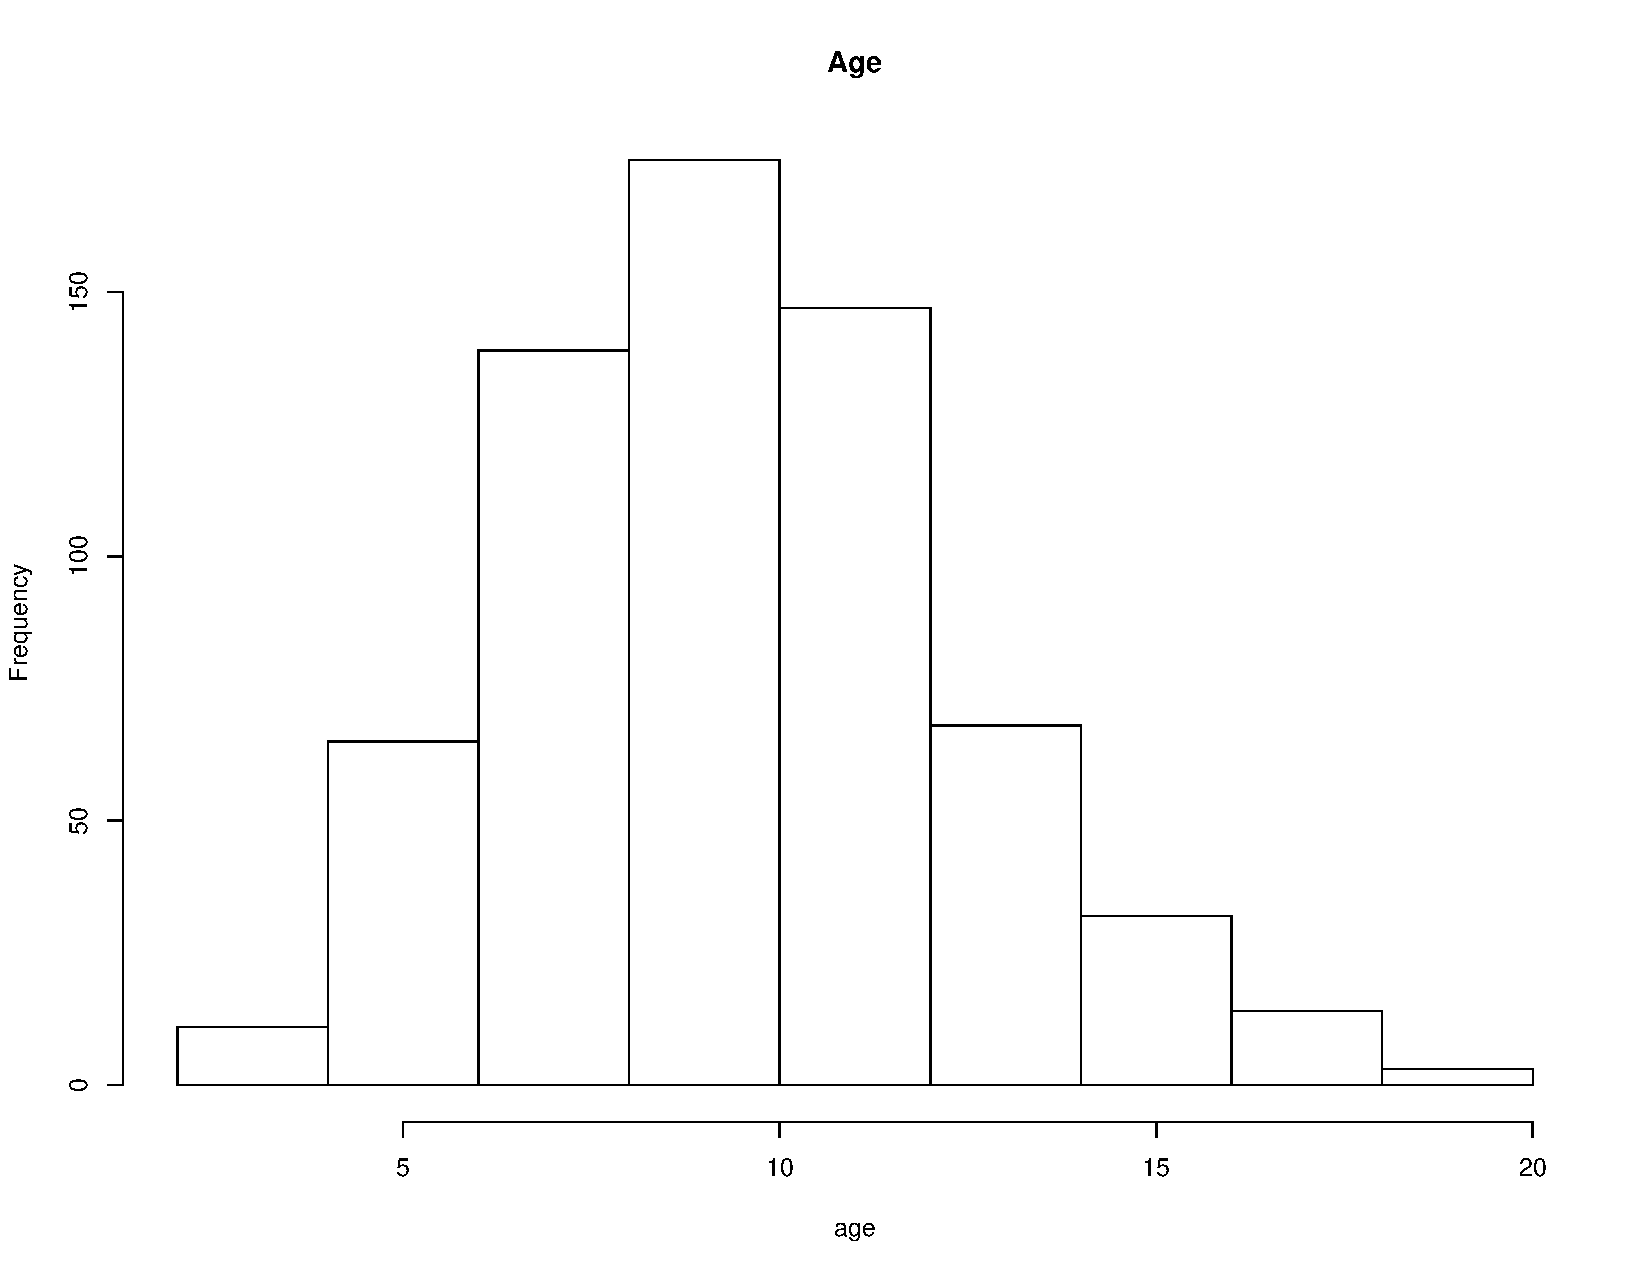
\includegraphics[width=4in, height=3.08in]{fevdoc-agehist}
\caption{Histogram of Age}
\label{agehist}
\end{figure}
\clearpage
\begin{Schunk}
\begin{Sinput}
> hist(height, main="Height")
\end{Sinput}
\end{Schunk}
\begin{figure}[h]
\centering
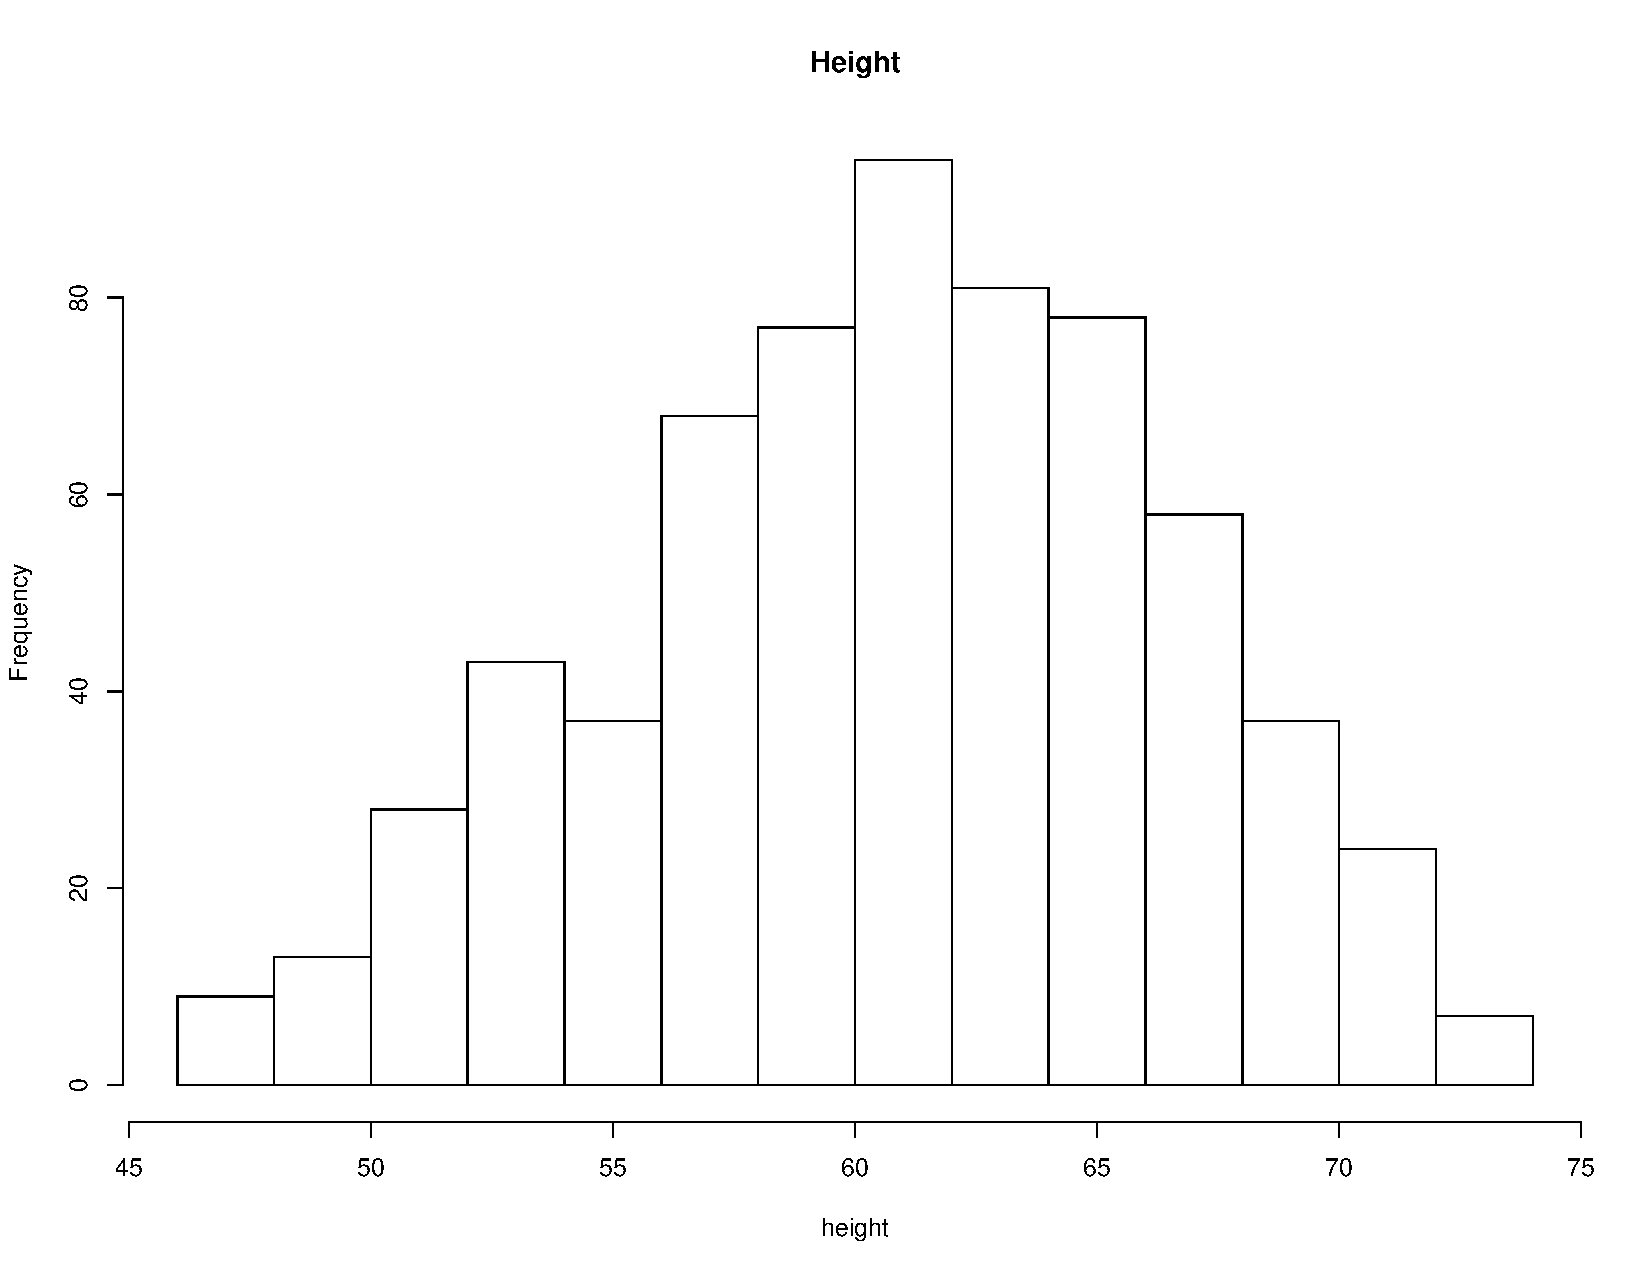
\includegraphics[width=4in, height=3.08in]{fevdoc-heighthist}
\caption{Histogram of Height}
\label{heighthist}
\end{figure}
\clearpage
\begin{Schunk}
\begin{Sinput}
> hist(fev, main="FEV")
\end{Sinput}
\end{Schunk}
\begin{figure}[h]
\centering
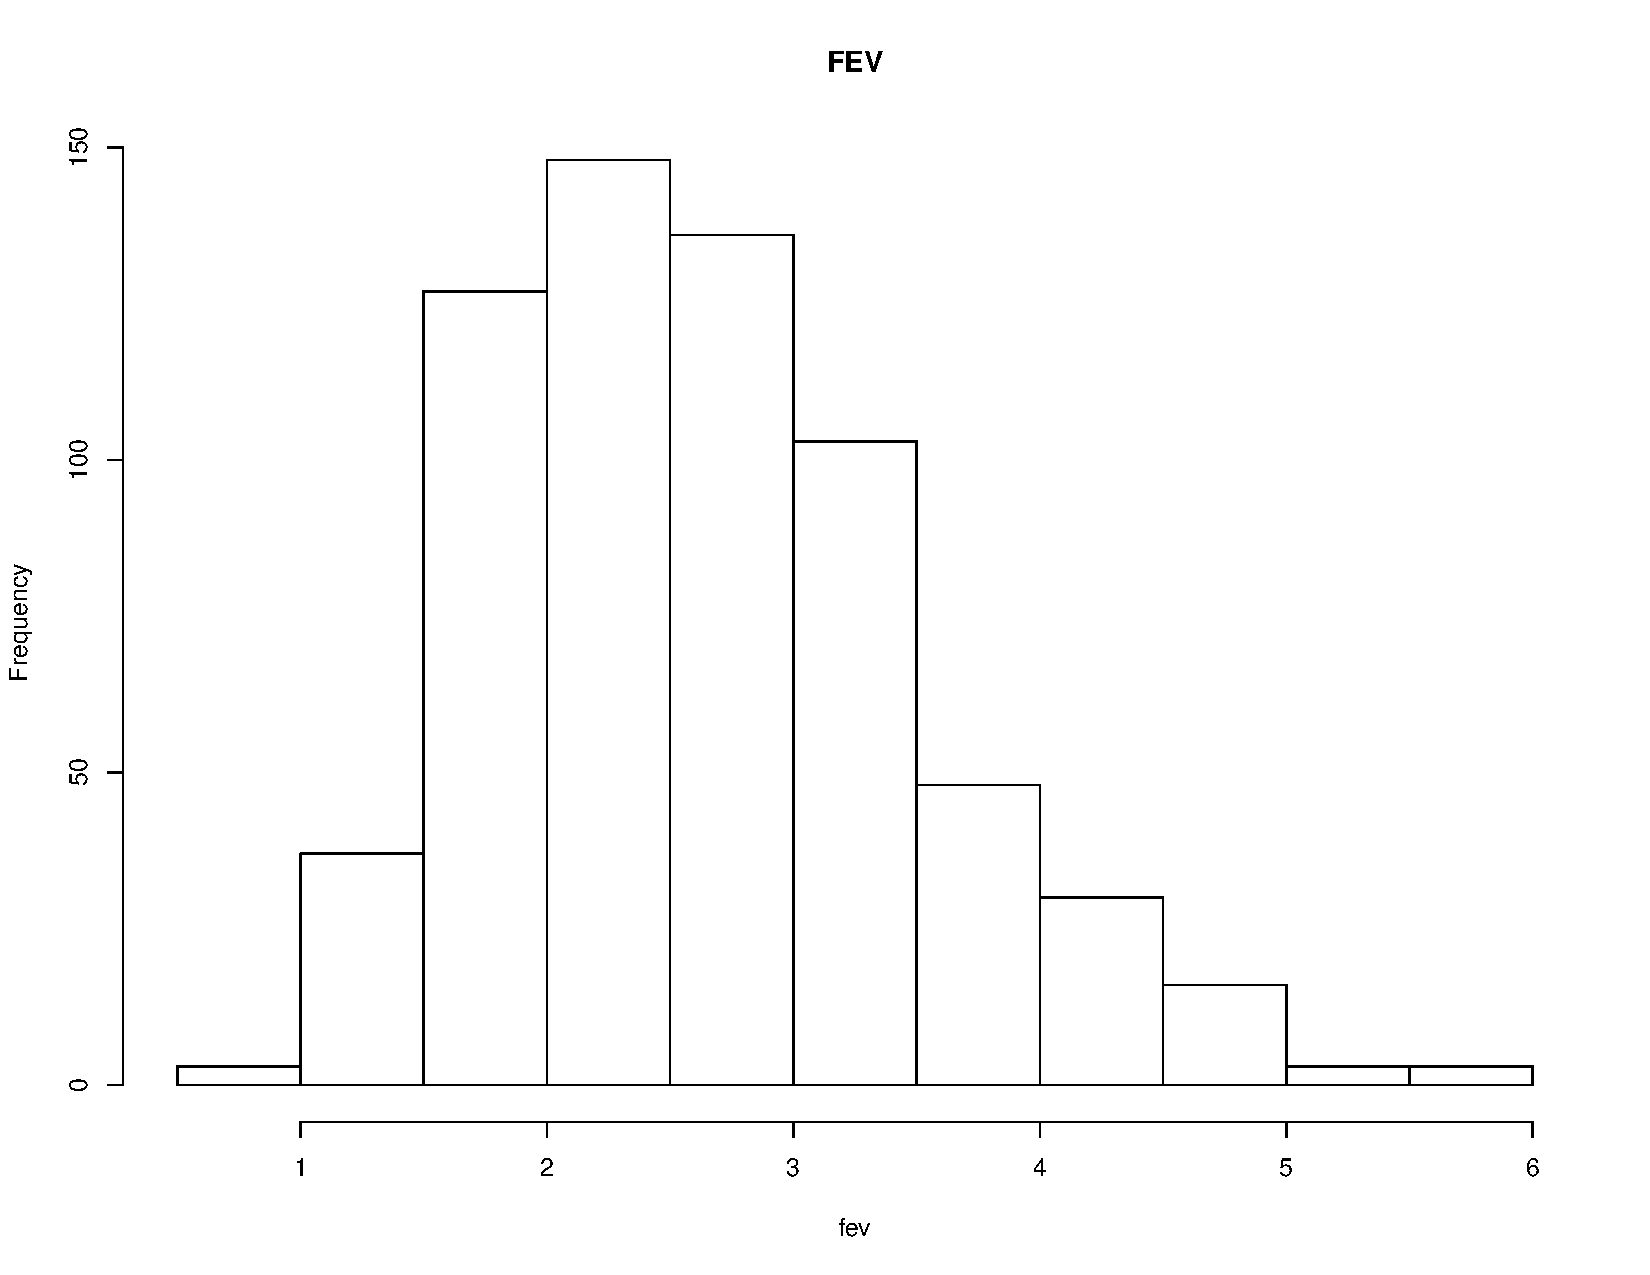
\includegraphics[width=4in, height=3.08in]{fevdoc-fevhist}
\caption{Histogram of FEV}
\label{fevhist}
\end{figure}
There is no bimodality in the data (each variable has only one peak) and thus we do not need to account for this in our analysis.
\clearpage
\subsection{Stratified descriptive statistics}
{\large \textbf{What do we want?}}\newline
Sometimes we believe that a variable has an effect on another. For example, we believe that sex has an effect on height. To see this effect, we need to stratify the height variable - that is, examine height in each sex individually. \newline
{\large \textbf{How do we do that?}}\newline
The \texttt{descrip()} function allows us to do this easily. We can stratify on any number of variables by adding them to the \texttt{strata} argument.\newline
{\large \textbf{Interpretation}}\newline
\begin{Schunk}
\begin{Sinput}
> descrip(age, height, strata=male)
\end{Sinput}
\begin{Soutput}
                  N     Msng  Mean      Std Dev    Min       25%       Mdn       75%       Max     
   age:  All        654     0   9.931     2.954     3.000     8.000     10.00     12.00     19.00  
   age:    Str  0   318     0   9.843     2.933     3.000     8.000     10.00     12.00     19.00  
   age:    Str  1   336     0   10.01     2.976     3.000     8.000     10.00     12.00     19.00  
height:  All        654     0   61.14     5.704     46.00     57.00     61.50     65.50     74.00  
height:    Str  0   318     0   60.21     4.792     46.00     57.50     61.00     63.50     71.00  
height:    Str  1   336     0   62.03     6.331     47.00     57.00     62.00     67.50     74.00  
\end{Soutput}
\end{Schunk}
\clearpage
\subsection{Box Plots}
{\large \textbf{What do we want?}}\newline
We want a graphical representation of the data with the mean, standard deviation, range, and potential outliers displayed. \newline
{\large \textbf{How do we do that?}}\newline
The \texttt{bplot()} function builds on the base R function \texttt{boxplot()}. Now we can add data, means, and standard deviations to the boxplot.\newline
{\large \textbf{Interpretation}}\newline
First, the na\"ive box plot for both age and height by sex - which means use the \texttt{male} variable (we only present code for the last plot, with the default values):\\
\begin{figure}[h]
\centering
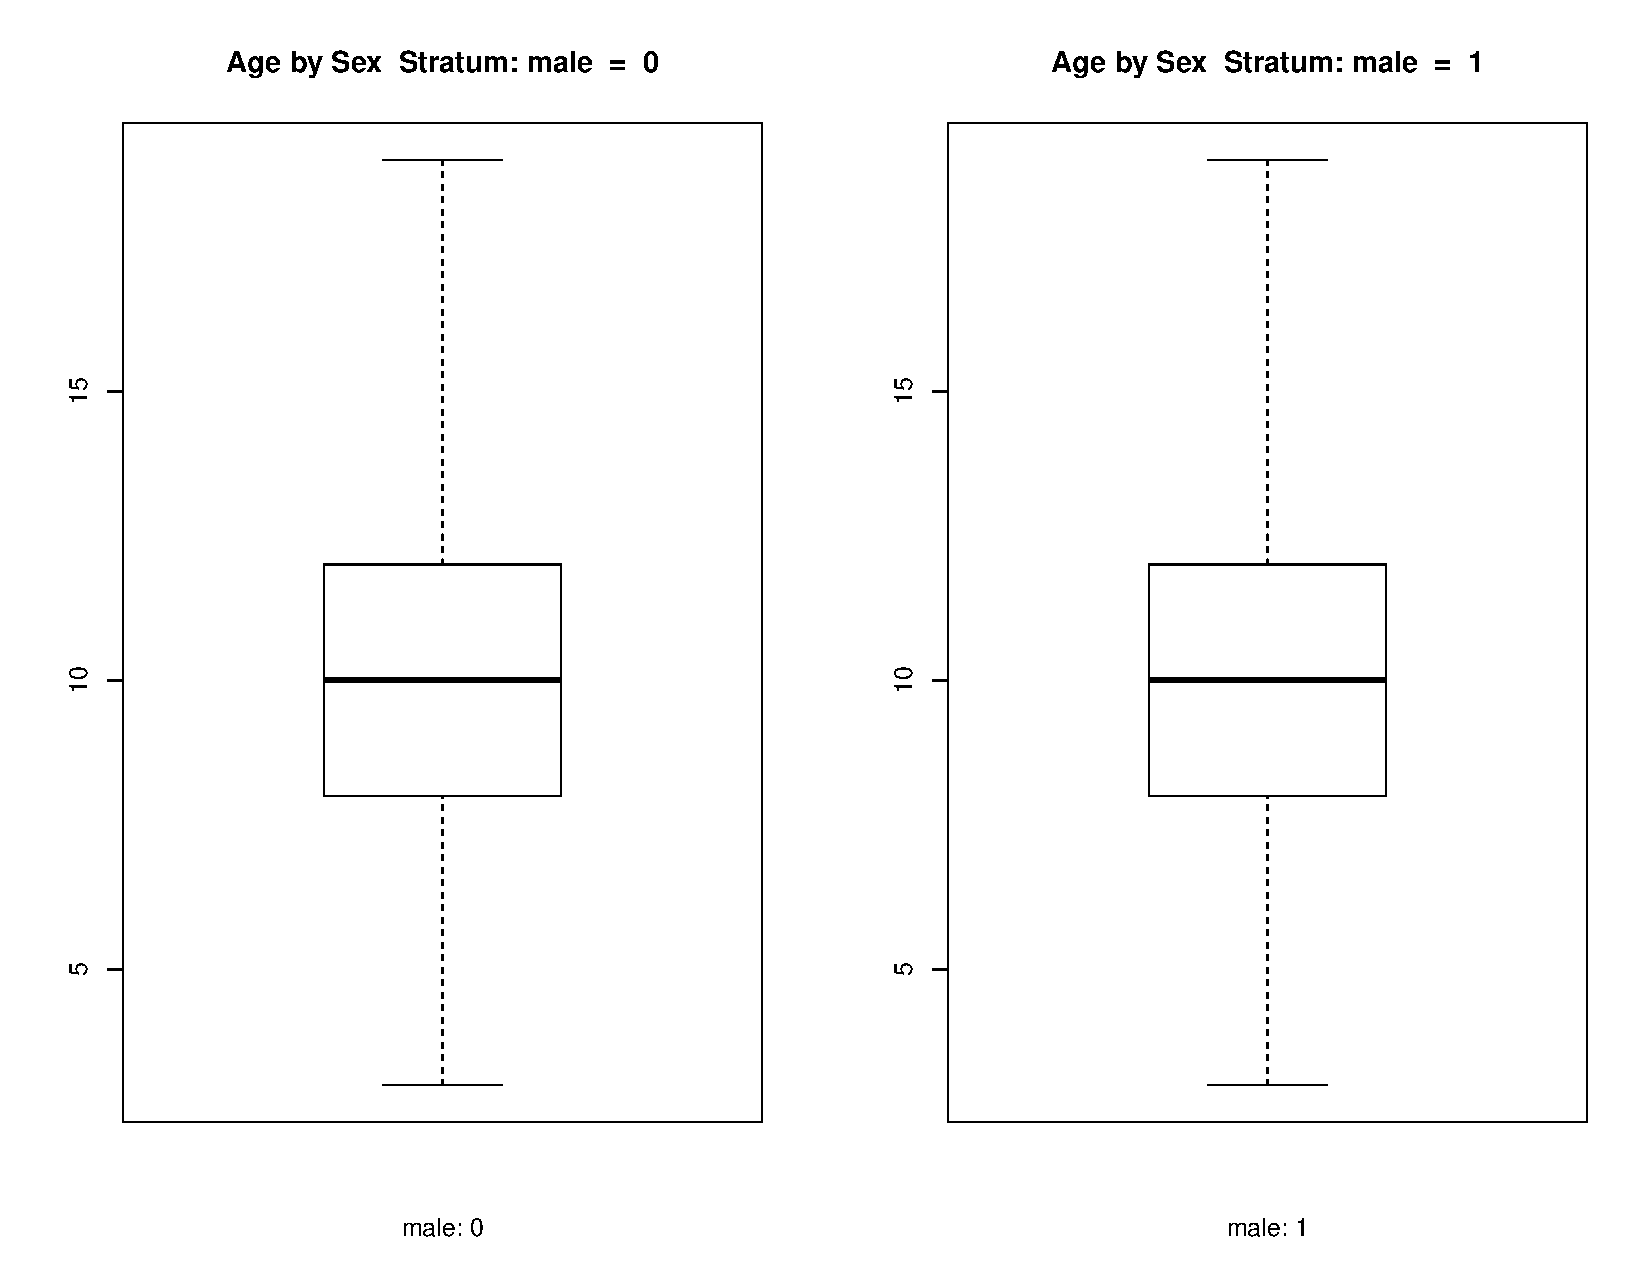
\includegraphics[width=4in, height=3.08in]{fevdoc-agebplot1}
\caption{Boxplot of Age by Sex}
\label{agebplot1}
\end{figure}
\clearpage
\begin{figure}[h]
\centering
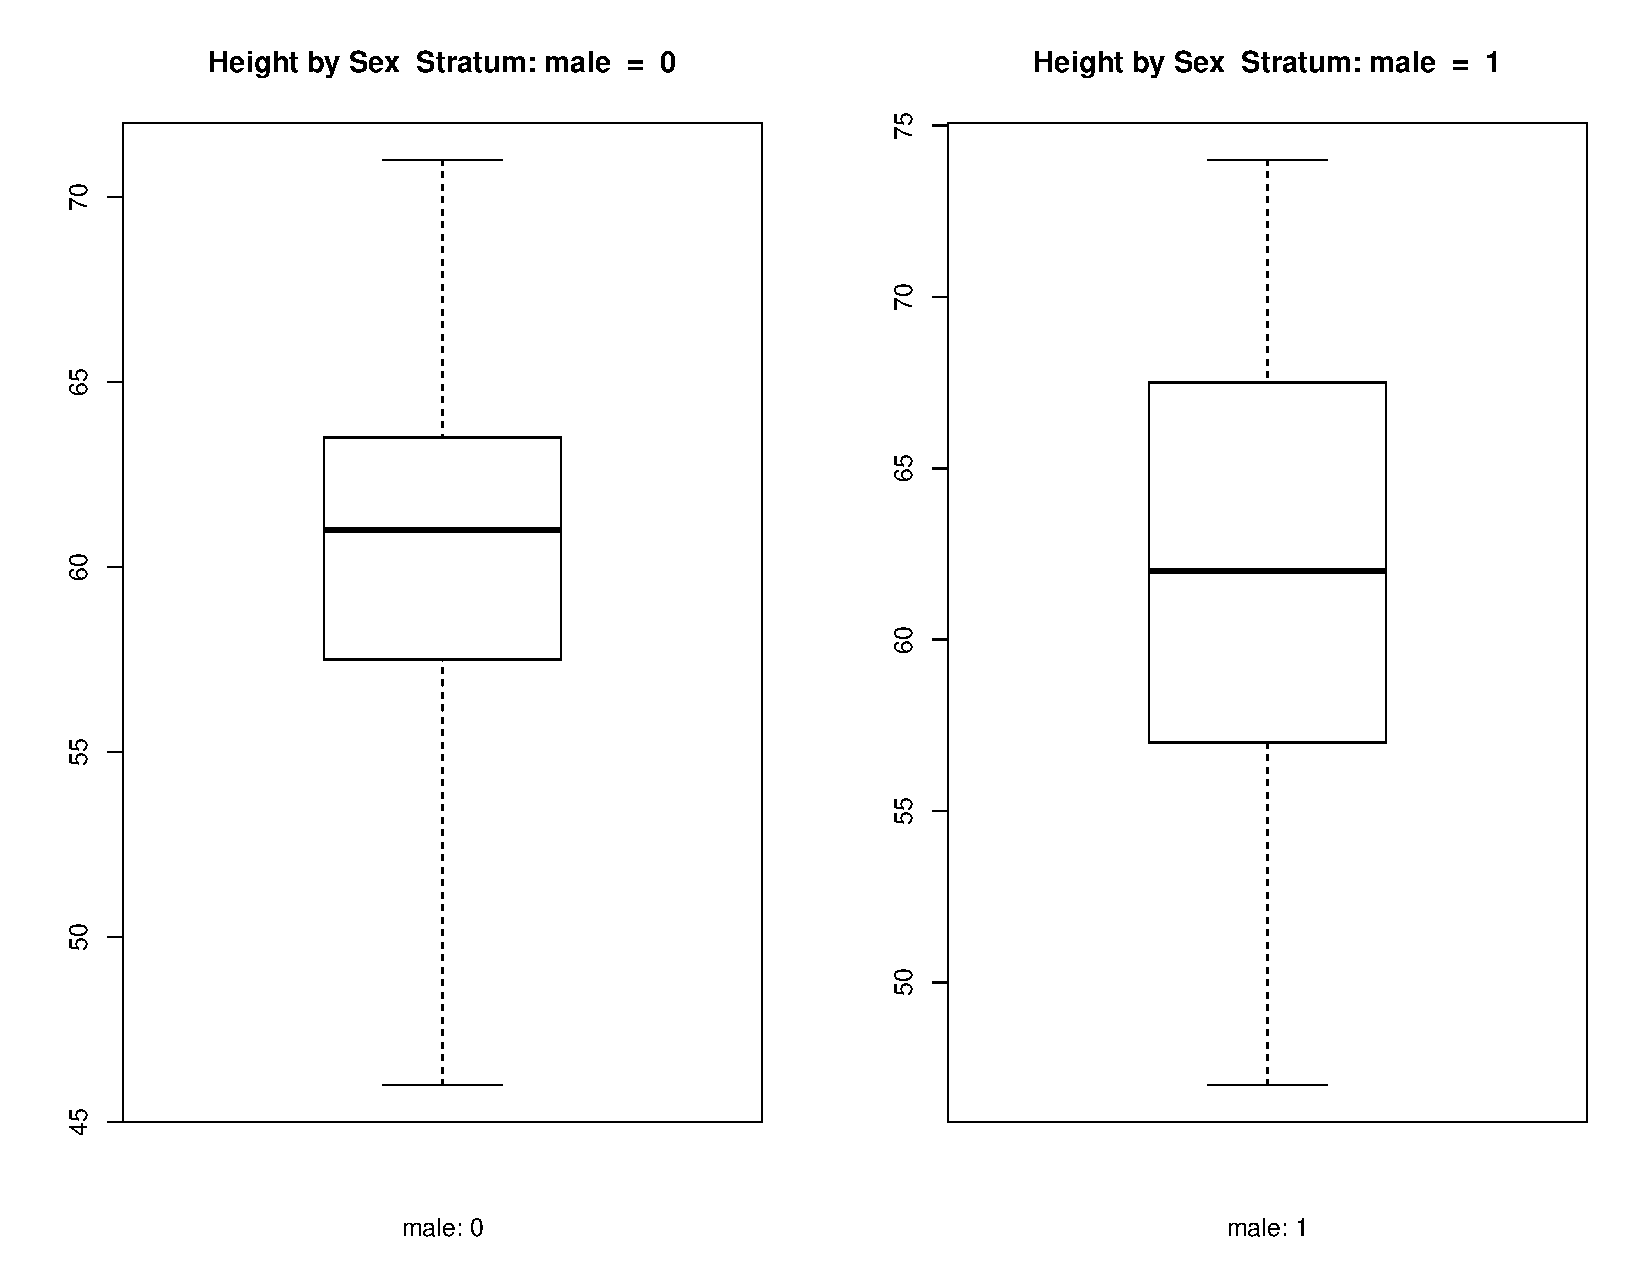
\includegraphics[width=4in, height=3.08in]{fevdoc-heightbplot1}
\caption{Boxplot of Height by Sex}
\label{heightbplot1}
\end{figure}
\clearpage
However, we can add jittered data to make this plot more informative (\texttt{bplot()} does this by default), and we can set the x-axis labels:\\
\begin{figure}[h]
\centering
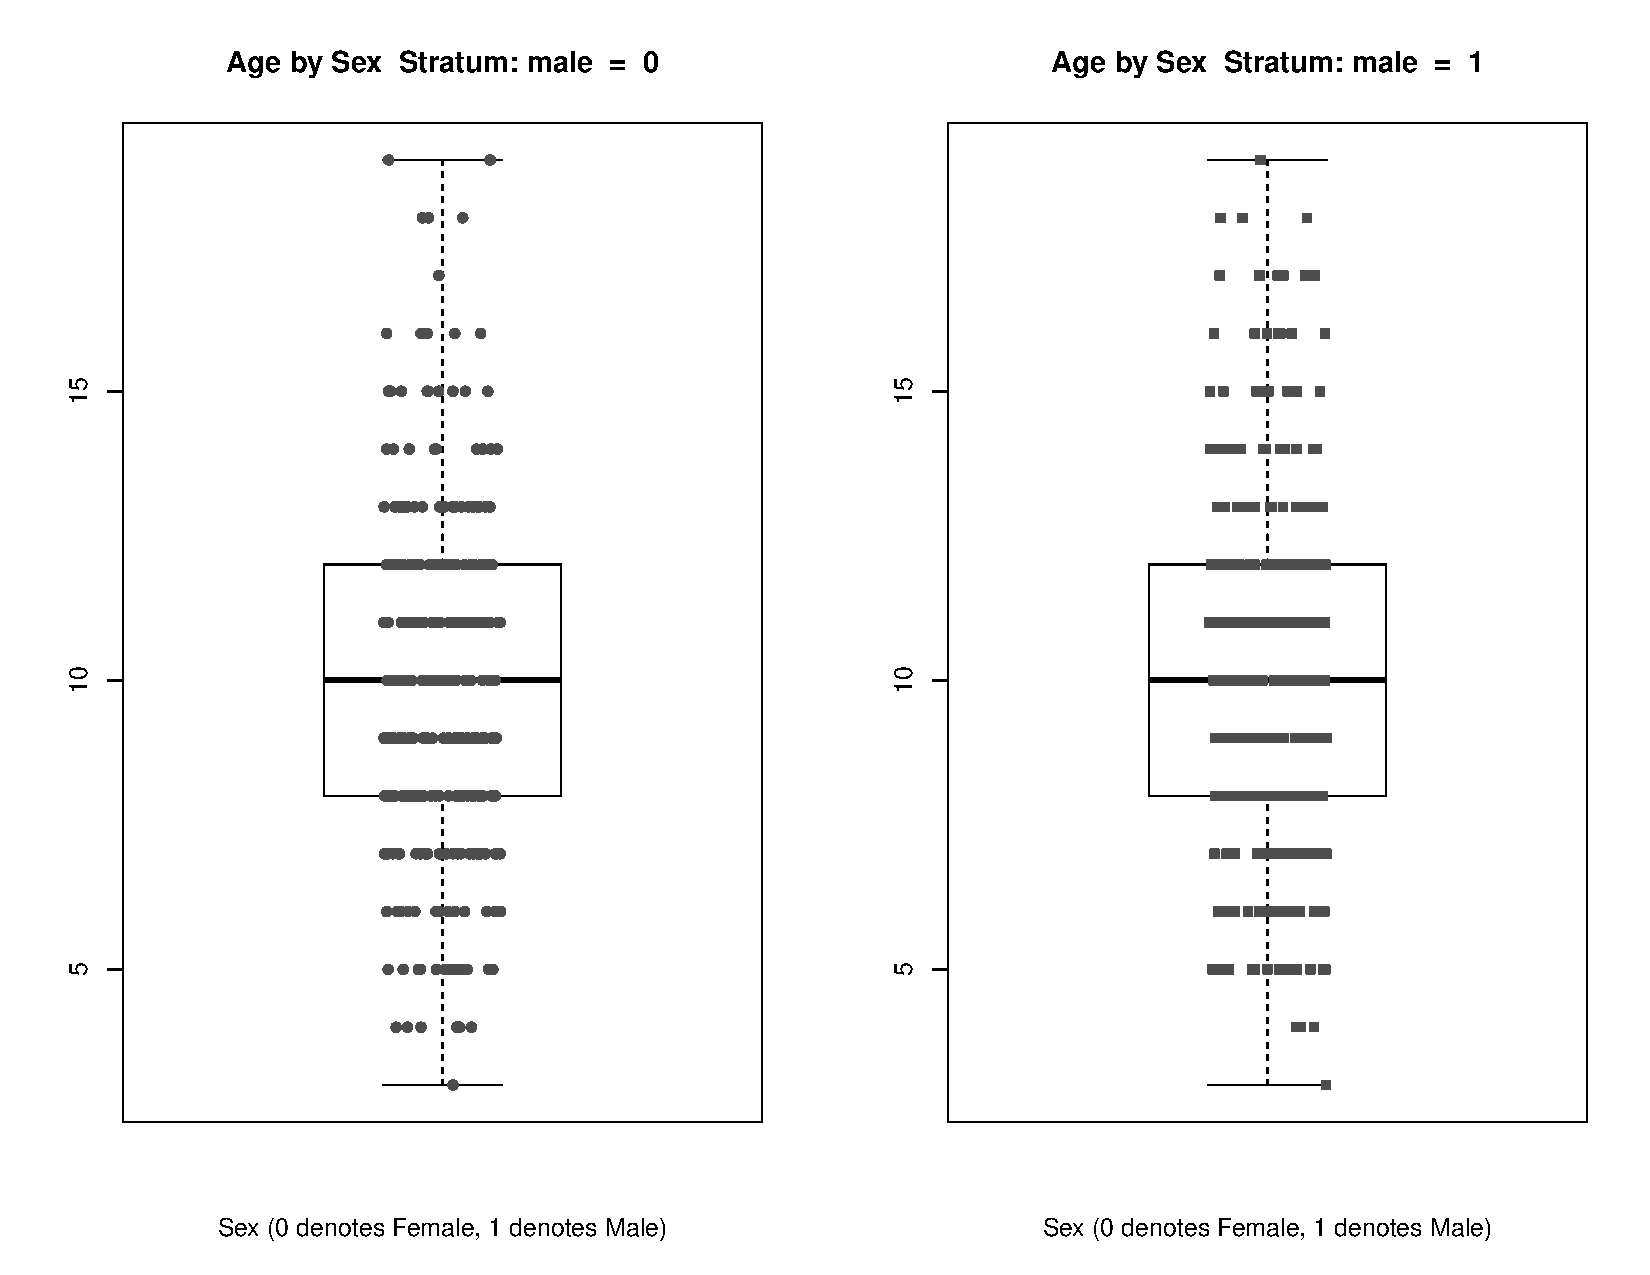
\includegraphics[width=4in, height=3.08in]{fevdoc-agebplot2}
\caption{Boxplot of Age by Sex with jittered data}
\label{agebplot2}
\end{figure}
\clearpage
\begin{figure}[h]
\centering
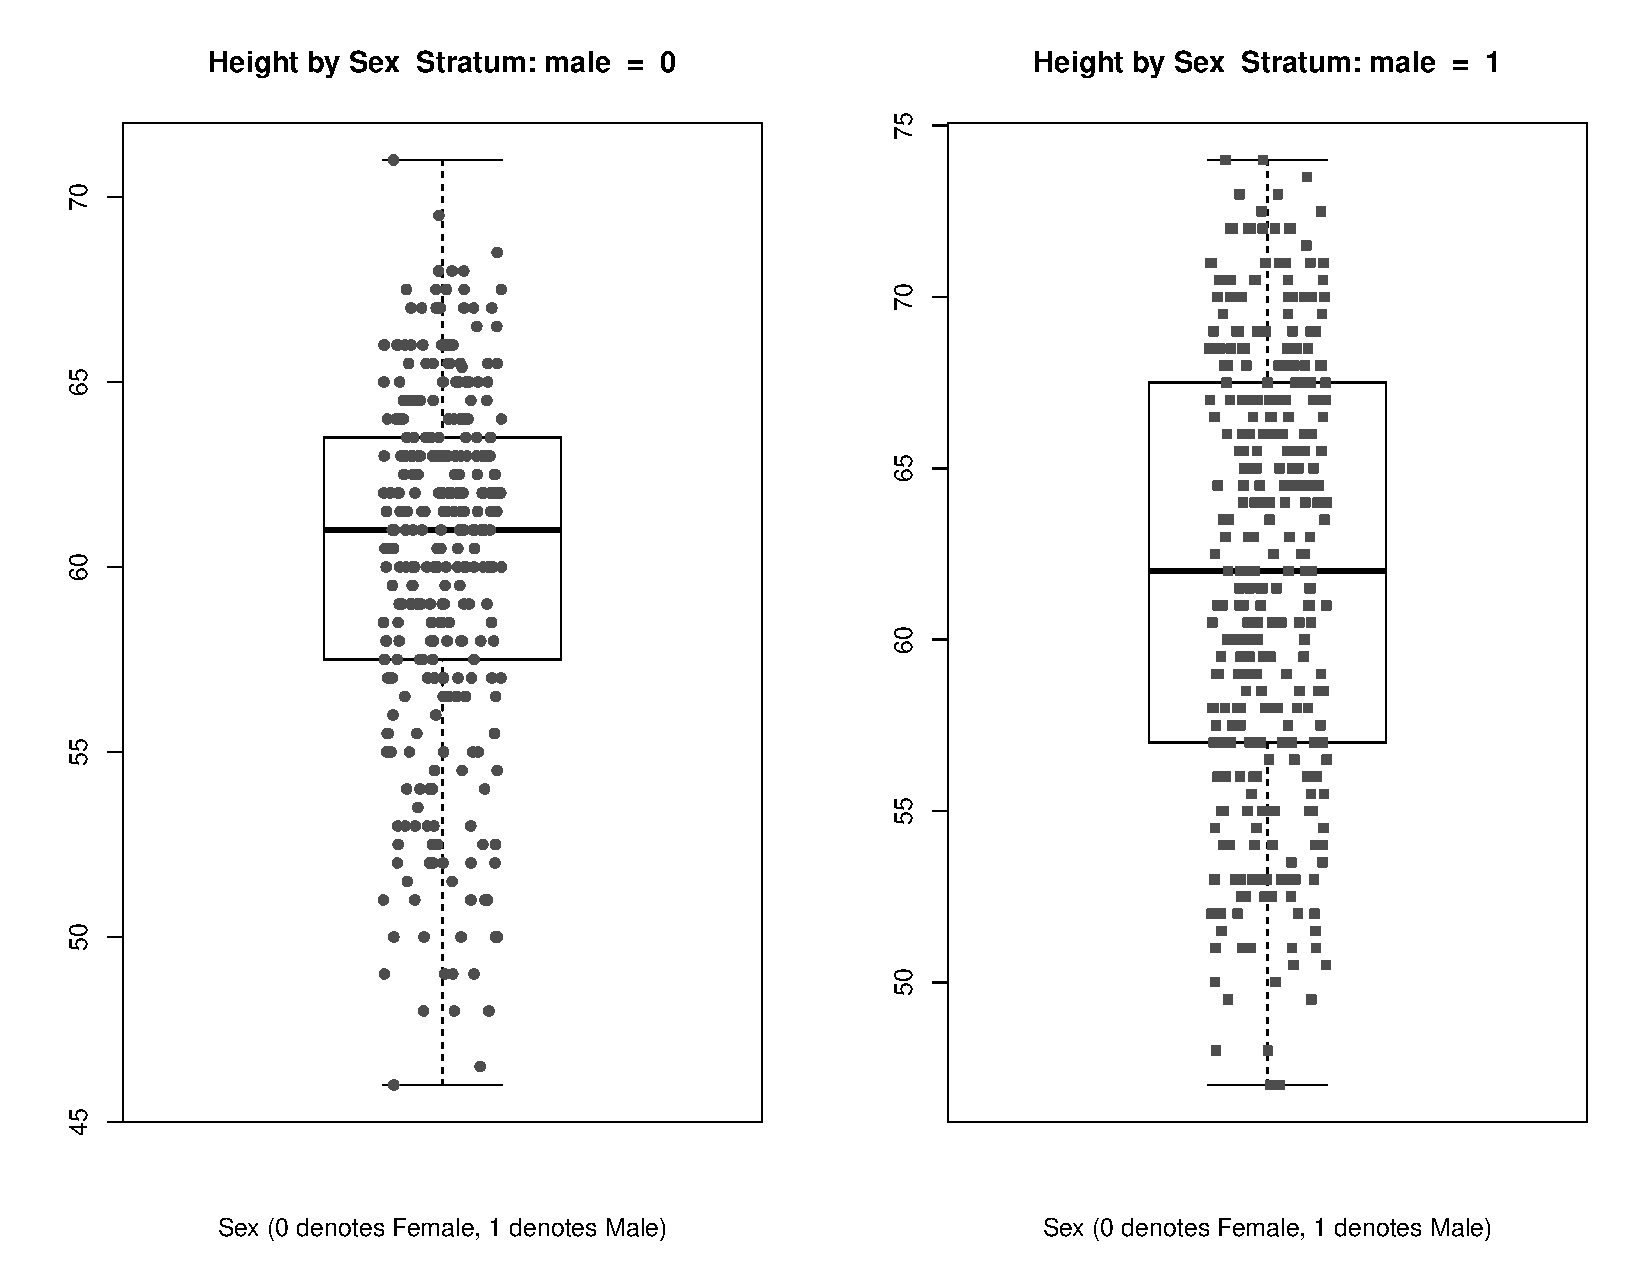
\includegraphics[width=4in, height=3.08in]{fevdoc-heightbplot2}
\caption{Boxplot of Height by Sex with jittered data}
\label{heightbplot2}
\end{figure}
\clearpage
We can also add the mean and standard deviation onto our box plot (\texttt{bplot()} does this by default as well) to get the maximum information from the plot:\\
\begin{Schunk}
\begin{Sinput}
> bplot(age, strata=male, main="Age by Sex", xlab="Sex (0 denotes Female, 1 denotes Male)")
\end{Sinput}
\end{Schunk}
\begin{figure}[h]
\centering
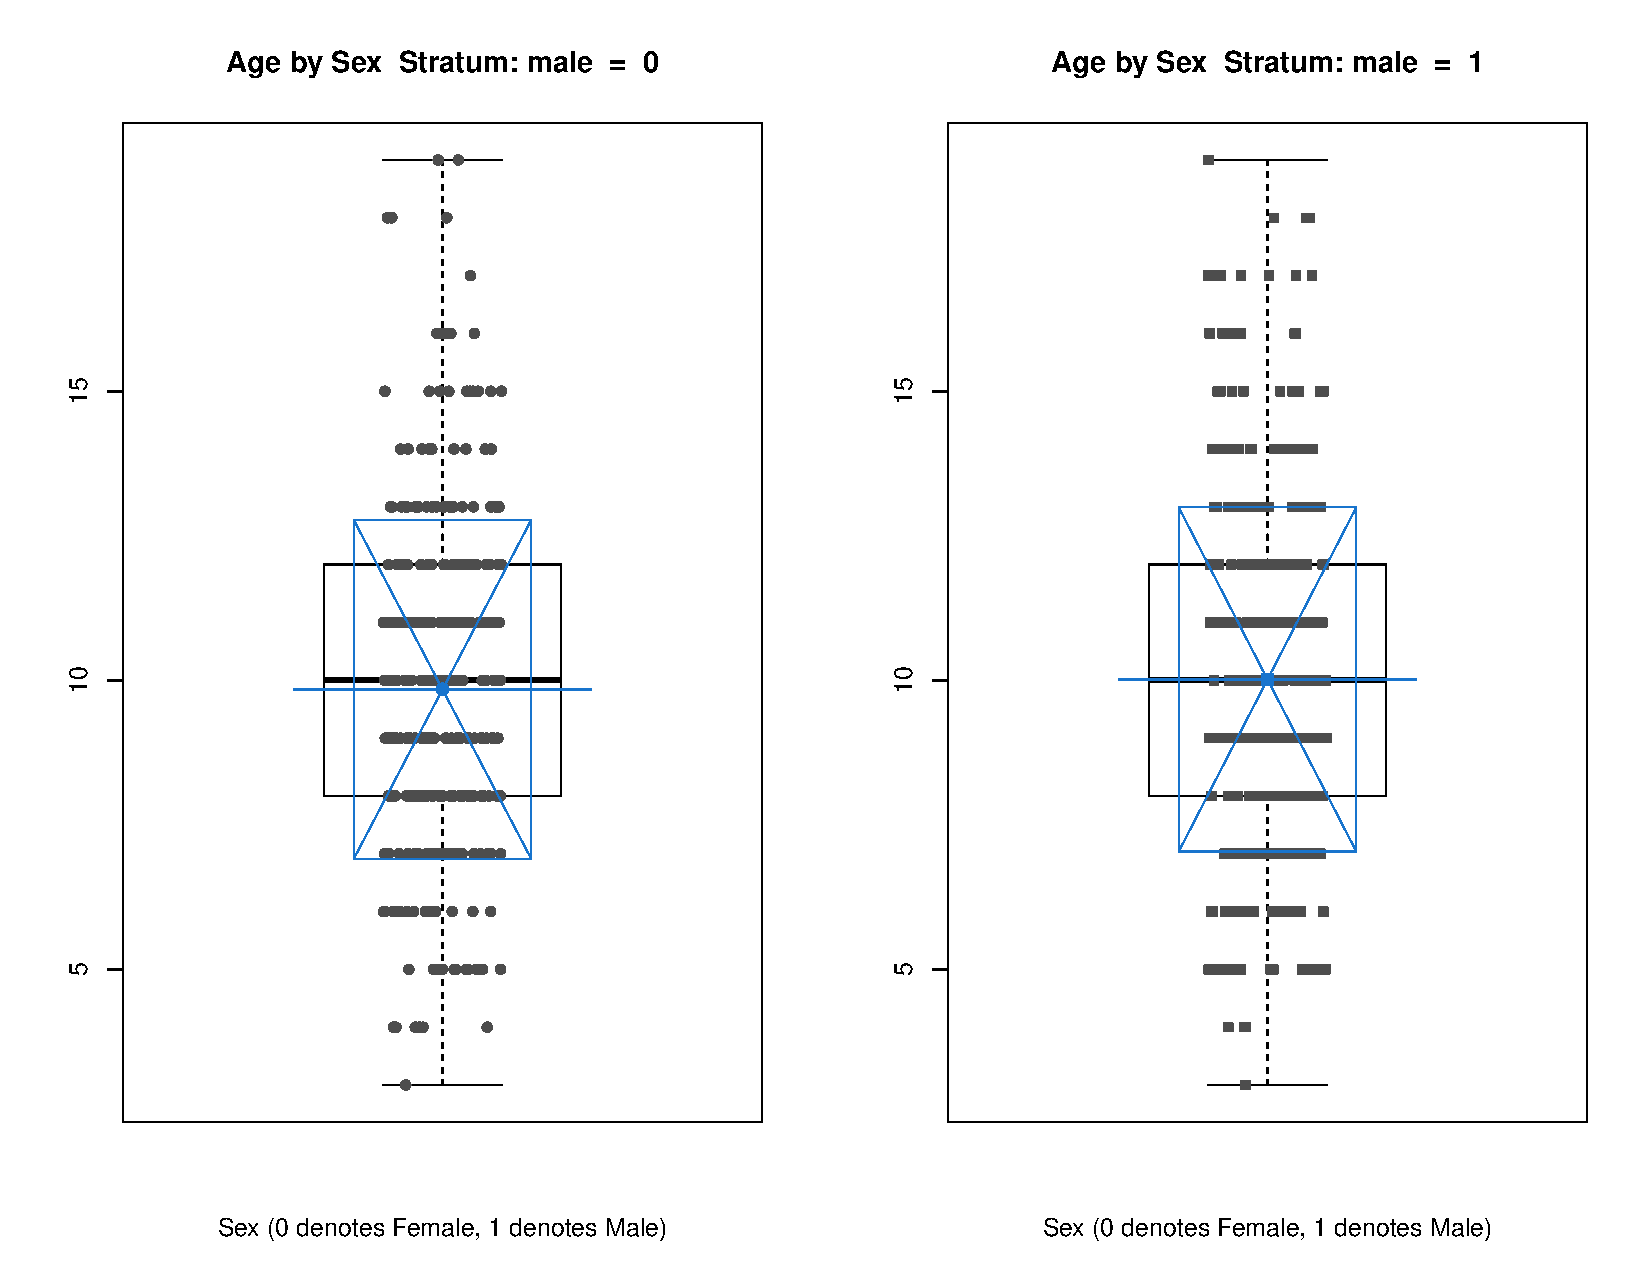
\includegraphics[width=4in, height=3.08in]{fevdoc-agebplot3}
\caption{Boxplot of Age by Sex with jittered data and mean and standard deviation overlaid}
\label{agebplot3}
\end{figure}
\clearpage
\begin{Schunk}
\begin{Sinput}
> bplot(height, strata=male, main="Height by Sex", xlab="Sex (0 denotes Female, 1 denotes Male)")
\end{Sinput}
\end{Schunk}
\begin{figure}[h]
\centering
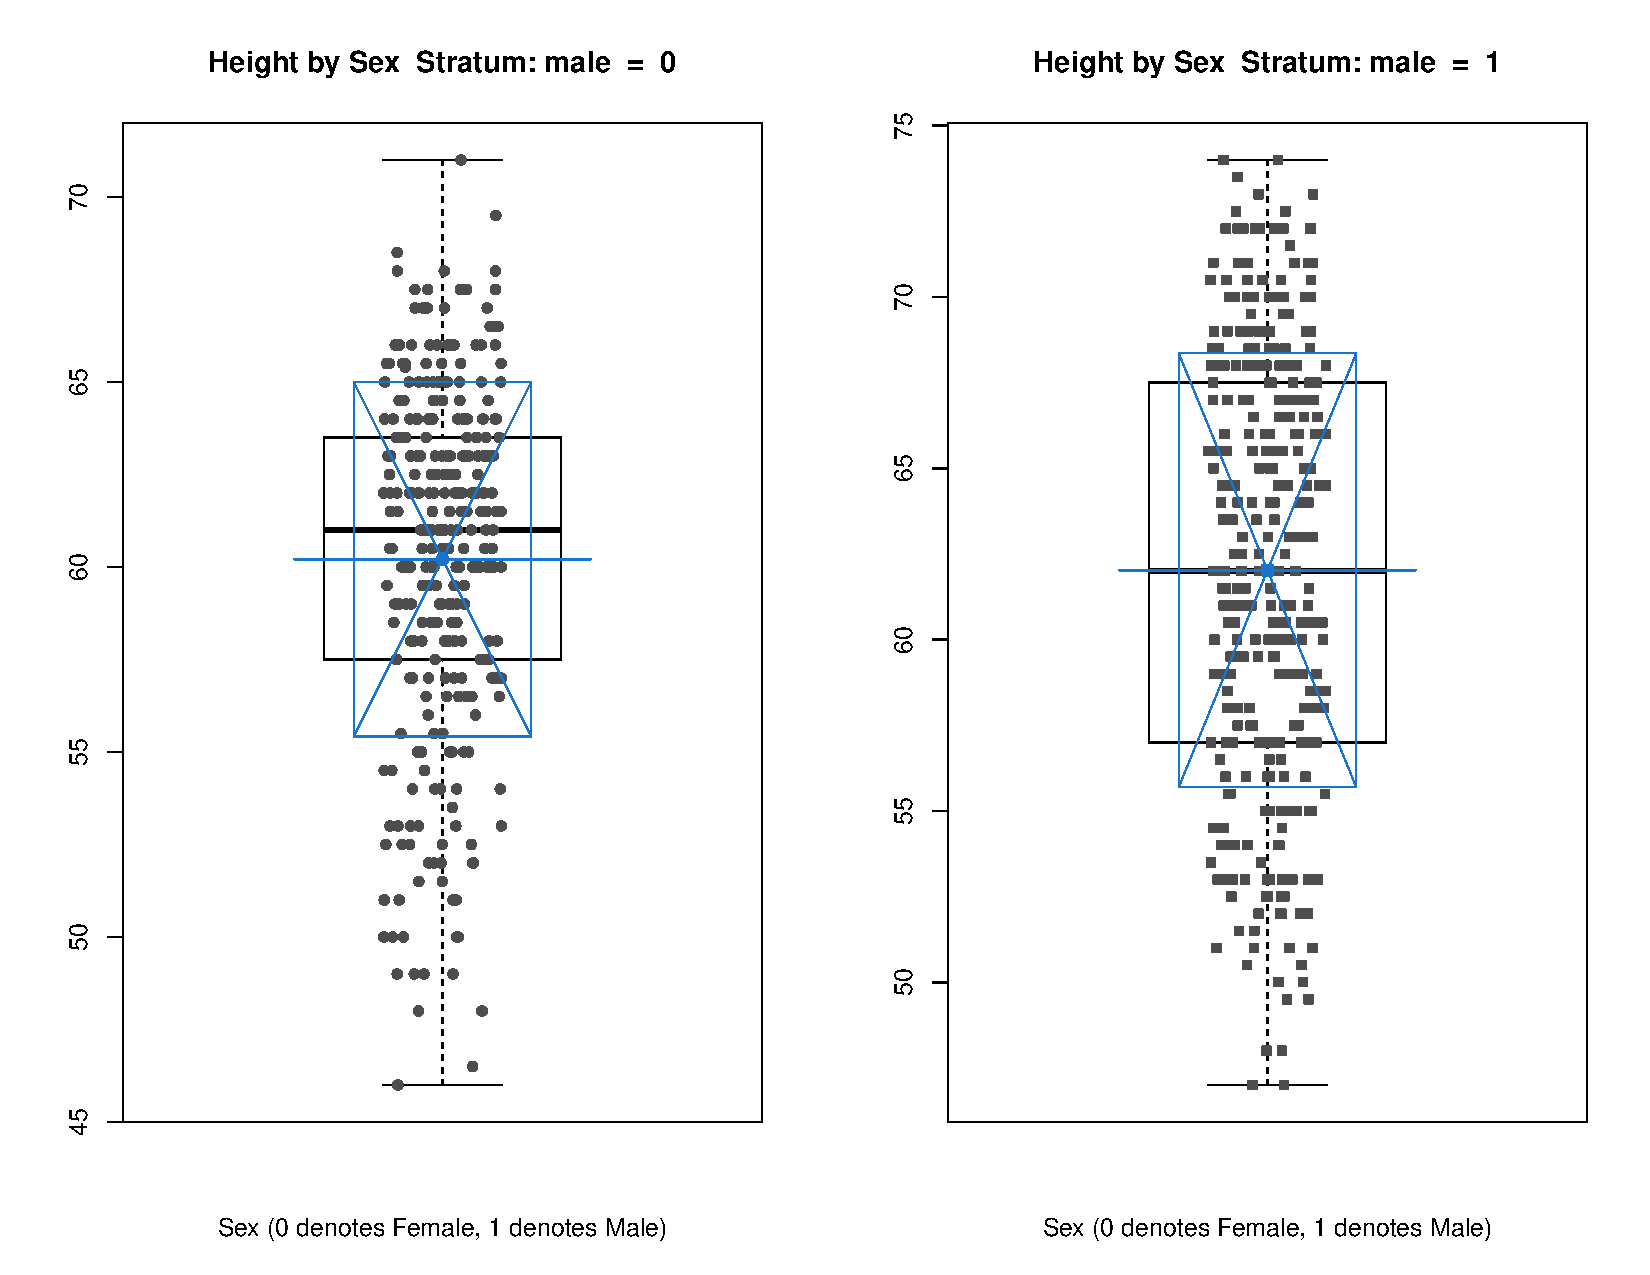
\includegraphics[width=4in, height=3.08in]{fevdoc-heightbplot3}
\caption{Boxplot of Height by Sex with jittered data and mean and standard deviation overlaid}
\label{heightbplot3}
\end{figure}
\clearpage
\subsection{Scatterplots}
Similar to the \texttt{bplot()} function, the \texttt{scatter()} function defaults to include some useful information. However, we will go through the derivation of the default values, so the only code shown will be the last (with defaults). The most basic version of the scatterplot does not differentiate between ties in the data (and thus we see much less than the 654 points on the plot):\\
\begin{figure}[h]
\centering
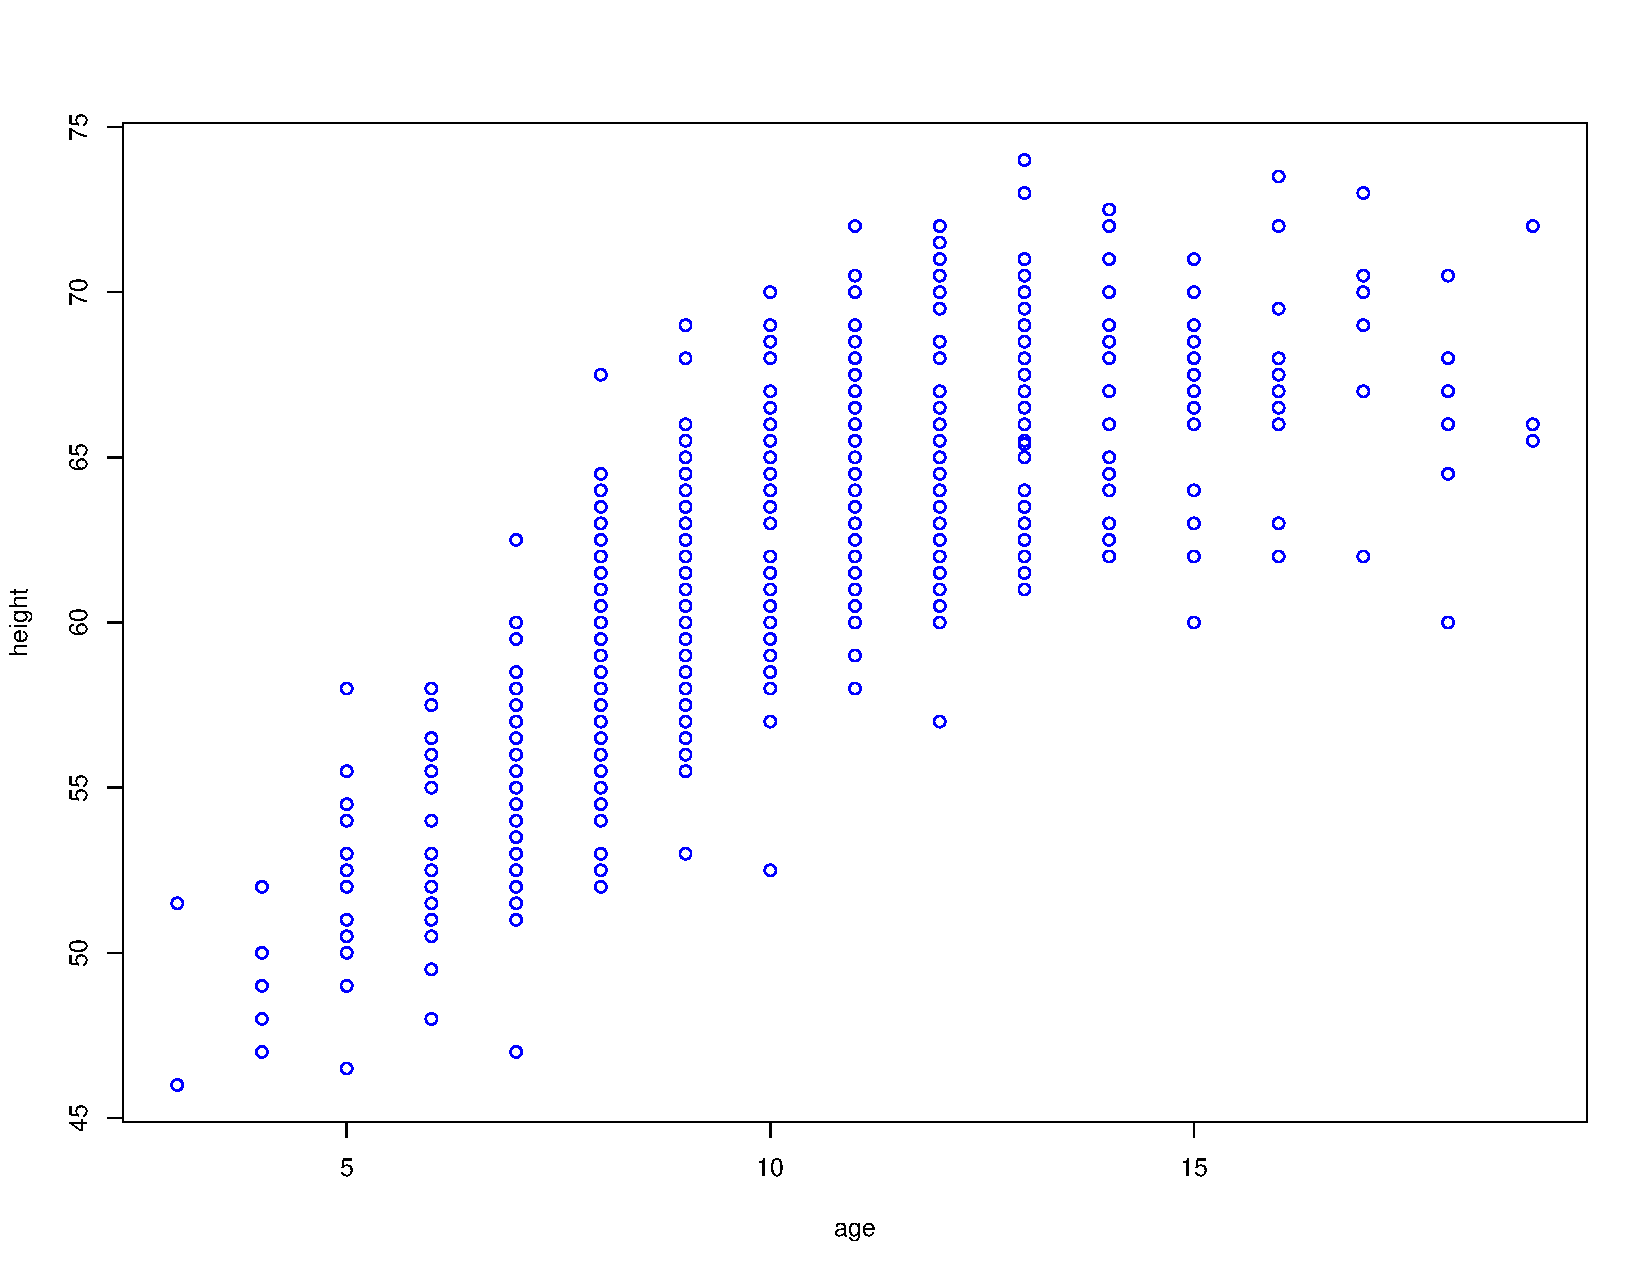
\includegraphics[scale=.005]{fevdoc-scatter1}
\caption{Scatterplot of Age vs Height}
\label{scatter1}
\end{figure}
However, we like to jitter the data so that we can see all of the points:\\
\begin{figure}[h]
\centering
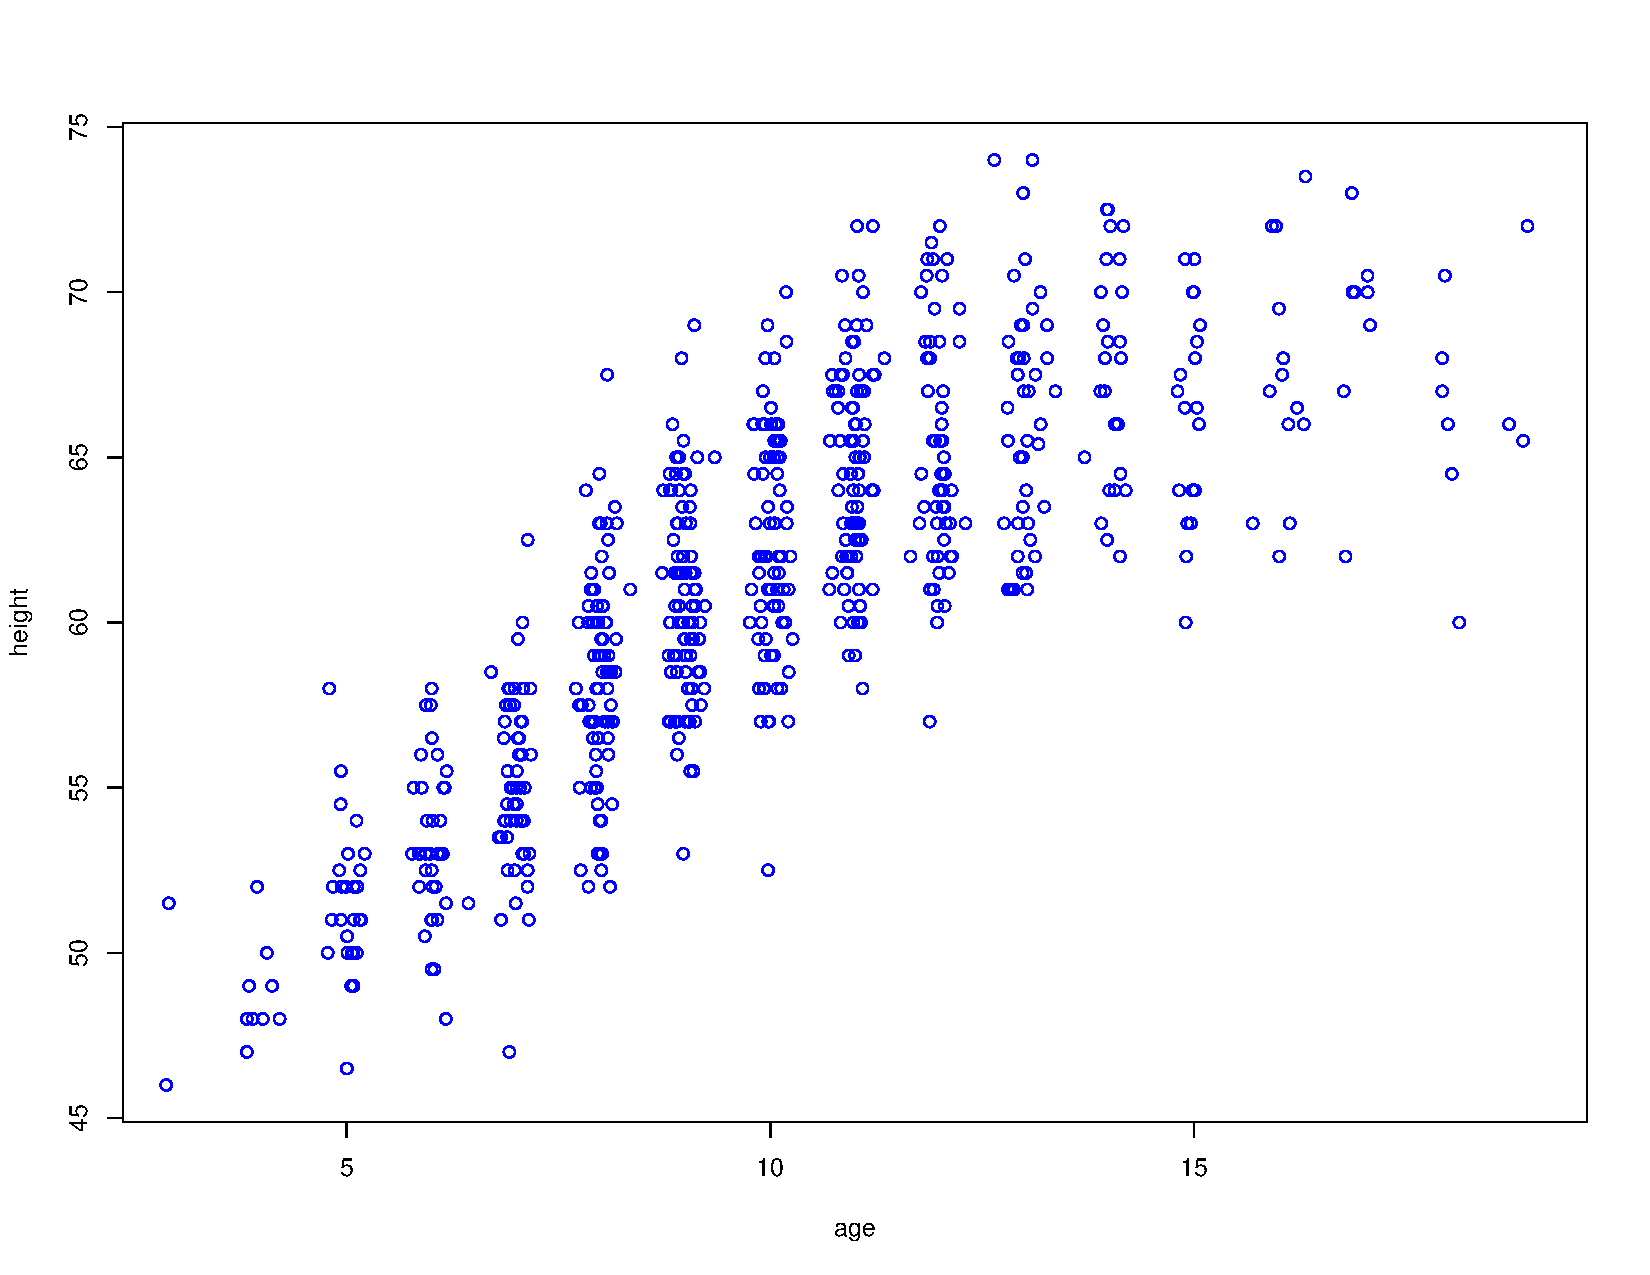
\includegraphics[scale=.005]{fevdoc-scatter2}
\caption{Scatterplot of Age vs Height with jittered data}
\label{scatter2}
\end{figure}
This allows us to break the ties and see all of the data, but still see the discreteness in the sampling. If we wanted to see a line of best fit, we could create one with the \texttt{plotLsfit} argument to our \texttt{scatter()} function:\\
\begin{figure}[h]
\centering
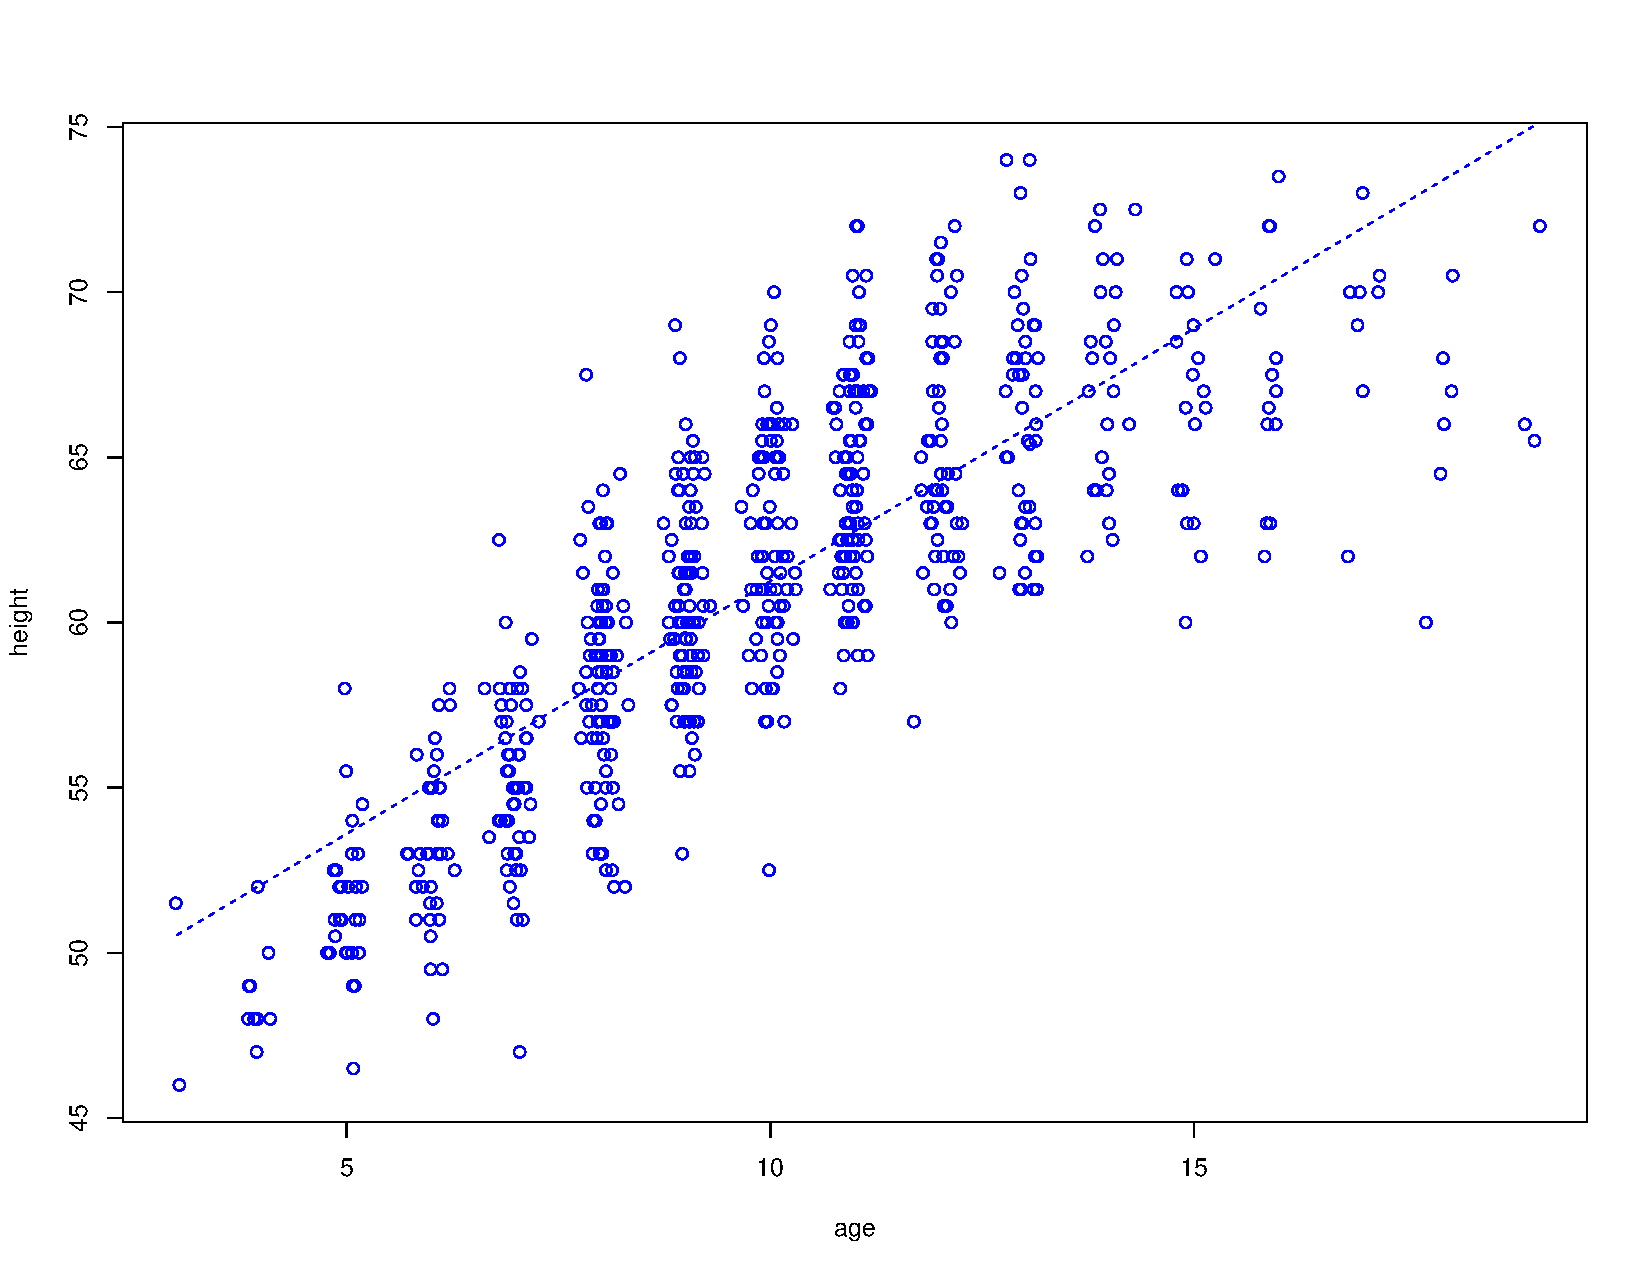
\includegraphics[scale=.005]{fevdoc-scatter3}
\caption{Scatterplot of Age vs Height with jittered data and least squares line}
\label{scatter3}
\end{figure}
If we look closely at the graph, the data doesn't look quite linear. We can solve this issue by plotting a lowess smooth, which will draw attention to the curves in the data:\\
\begin{Schunk}
\begin{Sinput}
> scatter(height, age)
\end{Sinput}
\end{Schunk}
\begin{figure}[h]
\centering
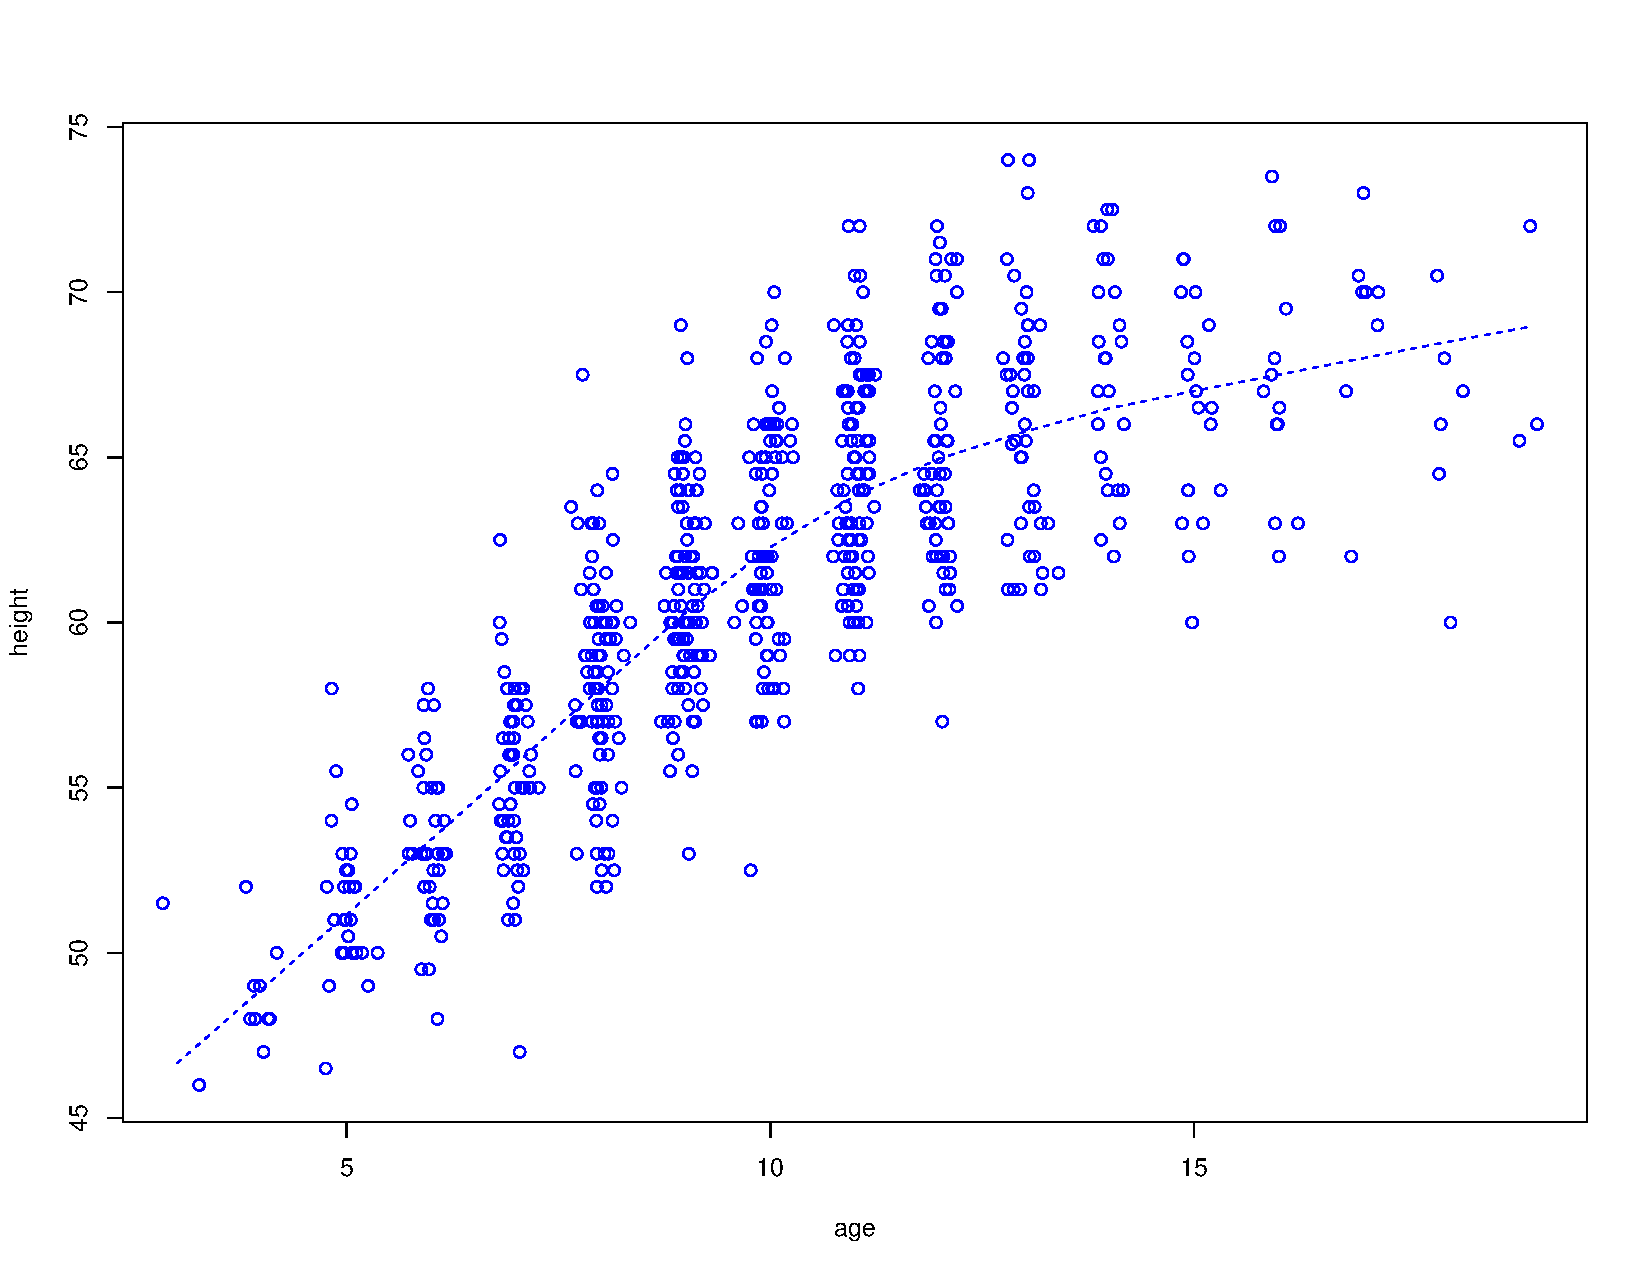
\includegraphics[scale=.005]{fevdoc-scatter4}
\caption{Scatterplot of Age vs Height with jittered data and lowess smooths}
\label{scatter4}
\end{figure}
\clearpage
\subsection{Confounding}
There might be potential confounders in the data. For instance, if smoking stunts growth, and only older kids smoke, then at higher ages we will have two populations separated by some vertical distance, while at lower ages we have only one population. It is generally useful to plot a stratified scatterplot with lowess smooths to check for confounders. By default, \texttt{scatter()} will use different colors for the strata. We can also label the axes and/or the graph:\\
\begin{Schunk}
\begin{Sinput}
> scatter(height, age, strata=smoker, main="Height vs Age by Smoking Status")
\end{Sinput}
\end{Schunk}
\begin{figure}[h]
\centering
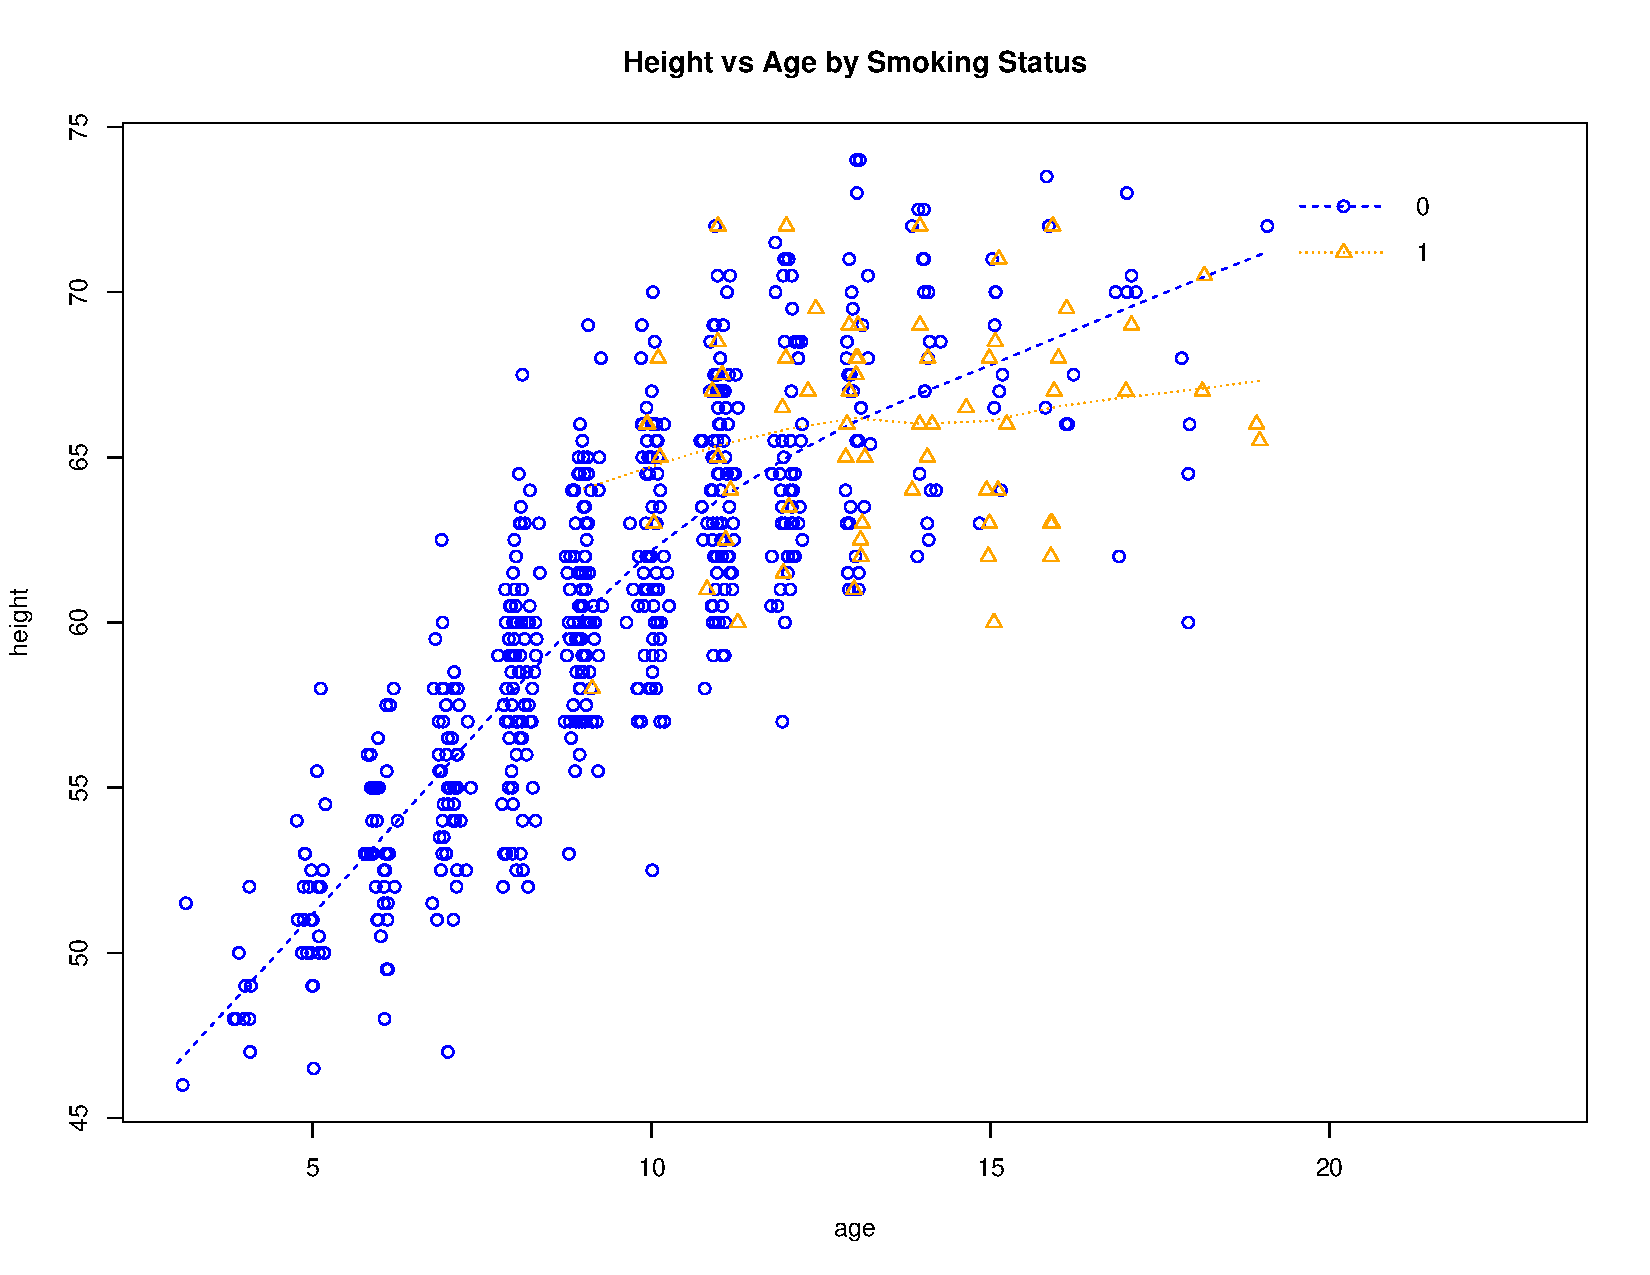
\includegraphics[scale=.005]{fevdoc-smokescatter}
\caption{Scatterplot of Age vs Height by Smoking Status}
\label{smokescatter}
\end{figure}
The legend gives us the color and type of point plotted for each stratum. Now if we wanted to see the lowess smooths for males and females, we can add them as a stratification variable: 
\begin{Schunk}
\begin{Sinput}
> scatter(height, age, strata=cbind(smoker, male), main="Height vs Age by Smoking Status")
\end{Sinput}
\end{Schunk}
\begin{figure}[h]
\centering
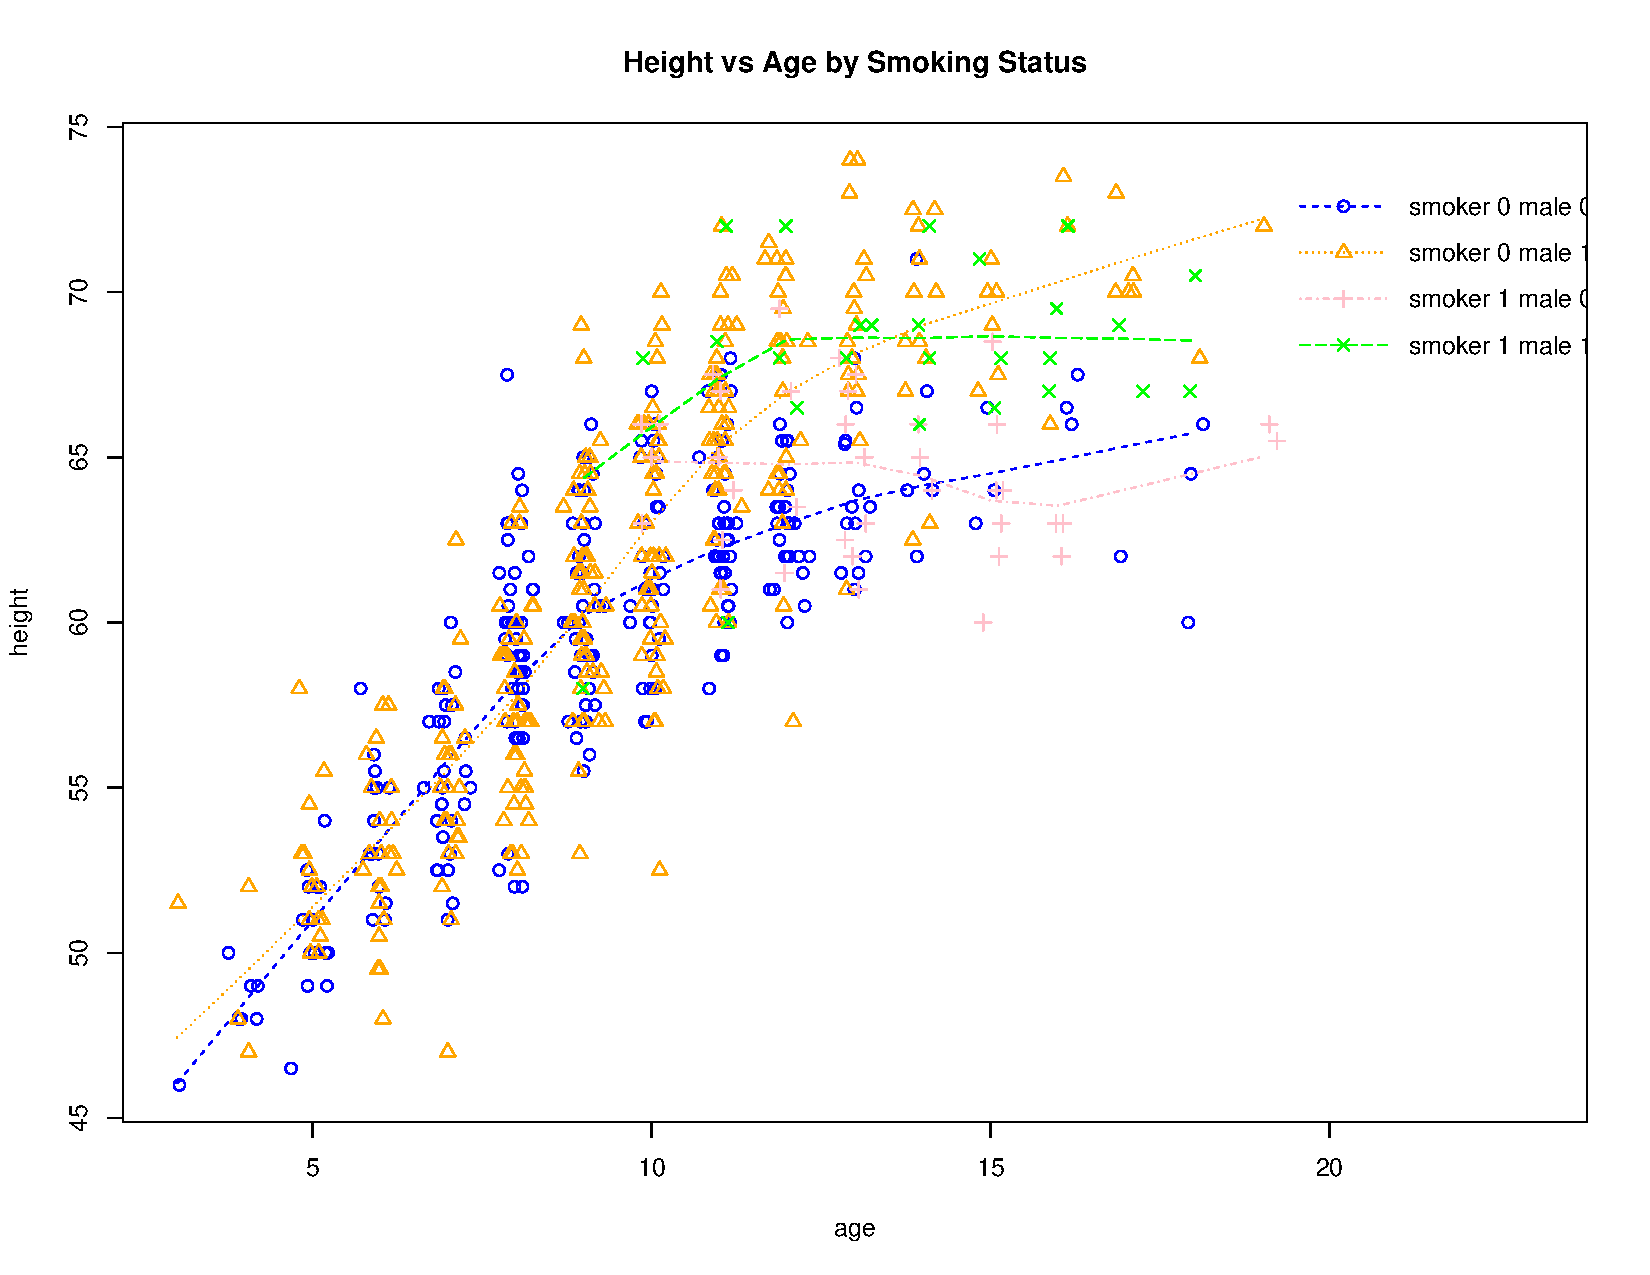
\includegraphics[scale=.005]{fevdoc-smokesexcatter}
\caption{Scatterplot of Age vs Height by Smoking Status and Sex}
\label{smokesexcatter}
\end{figure}
Now notice that we can compare groups both across sex (\texttt{sex 1} is male and \texttt{sex 2} is female) or across smoking. 
\clearpage
\subsection{Trends and Transforming the Data}
Convinced that smoking is not too much of a confounder, we now look at age vs fev. If we do so first with no lowess smooth, it is hard to tell what the trend in the data is:\\
\begin{Schunk}
\begin{Sinput}
> scatter(fev, age, plotLowess=FALSE, main="FEV vs Age")
\end{Sinput}
\end{Schunk}
\begin{figure}[h]
\centering
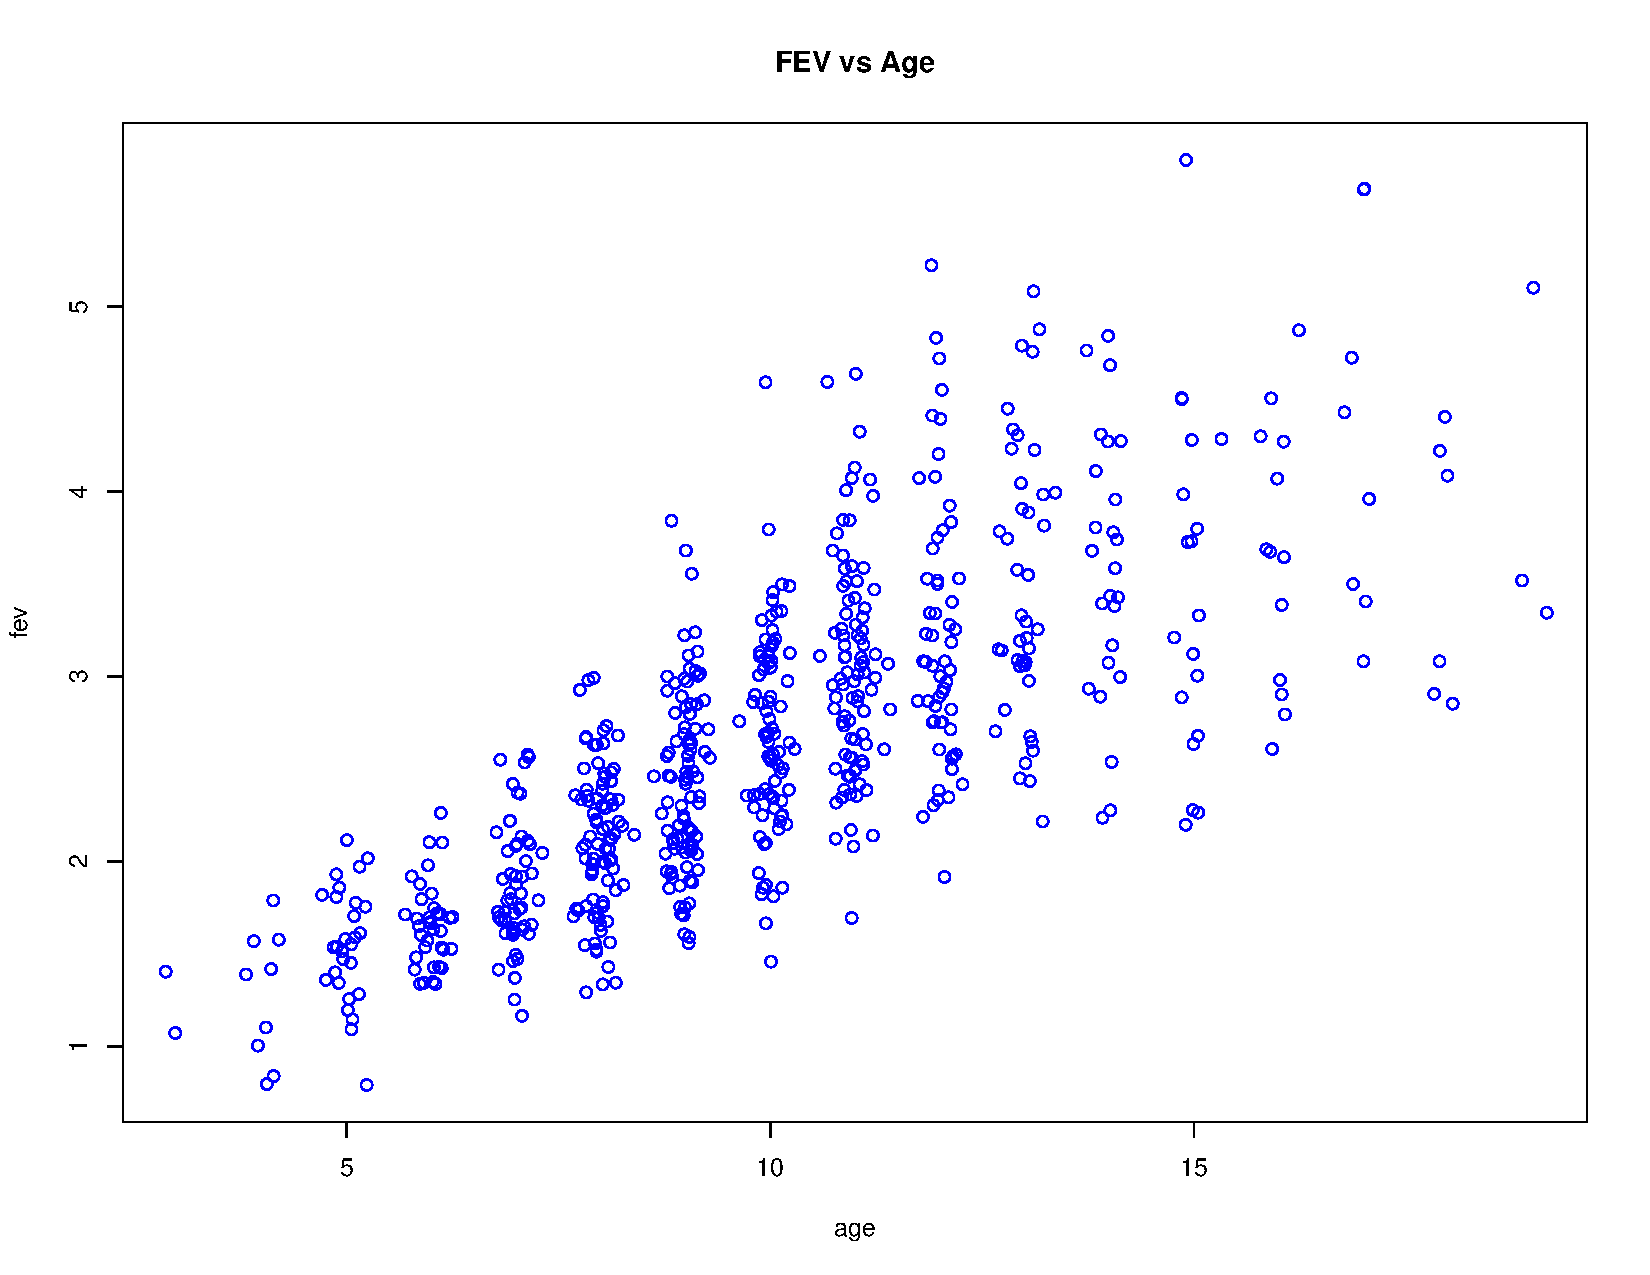
\includegraphics[scale=.005]{fevdoc-agefevscatter}
\caption{Scatterplot of Age vs Height}
\label{agefevscatter}
\end{figure}Any pattern is incredibly hard to find. We might think that the data is linear, but putting a lowess smooth on the plot shows us differently:\\
\begin{Schunk}
\begin{Sinput}
> scatter(fev, age, main="FEV vs Age")
\end{Sinput}
\end{Schunk}
\begin{figure}[h]
\centering
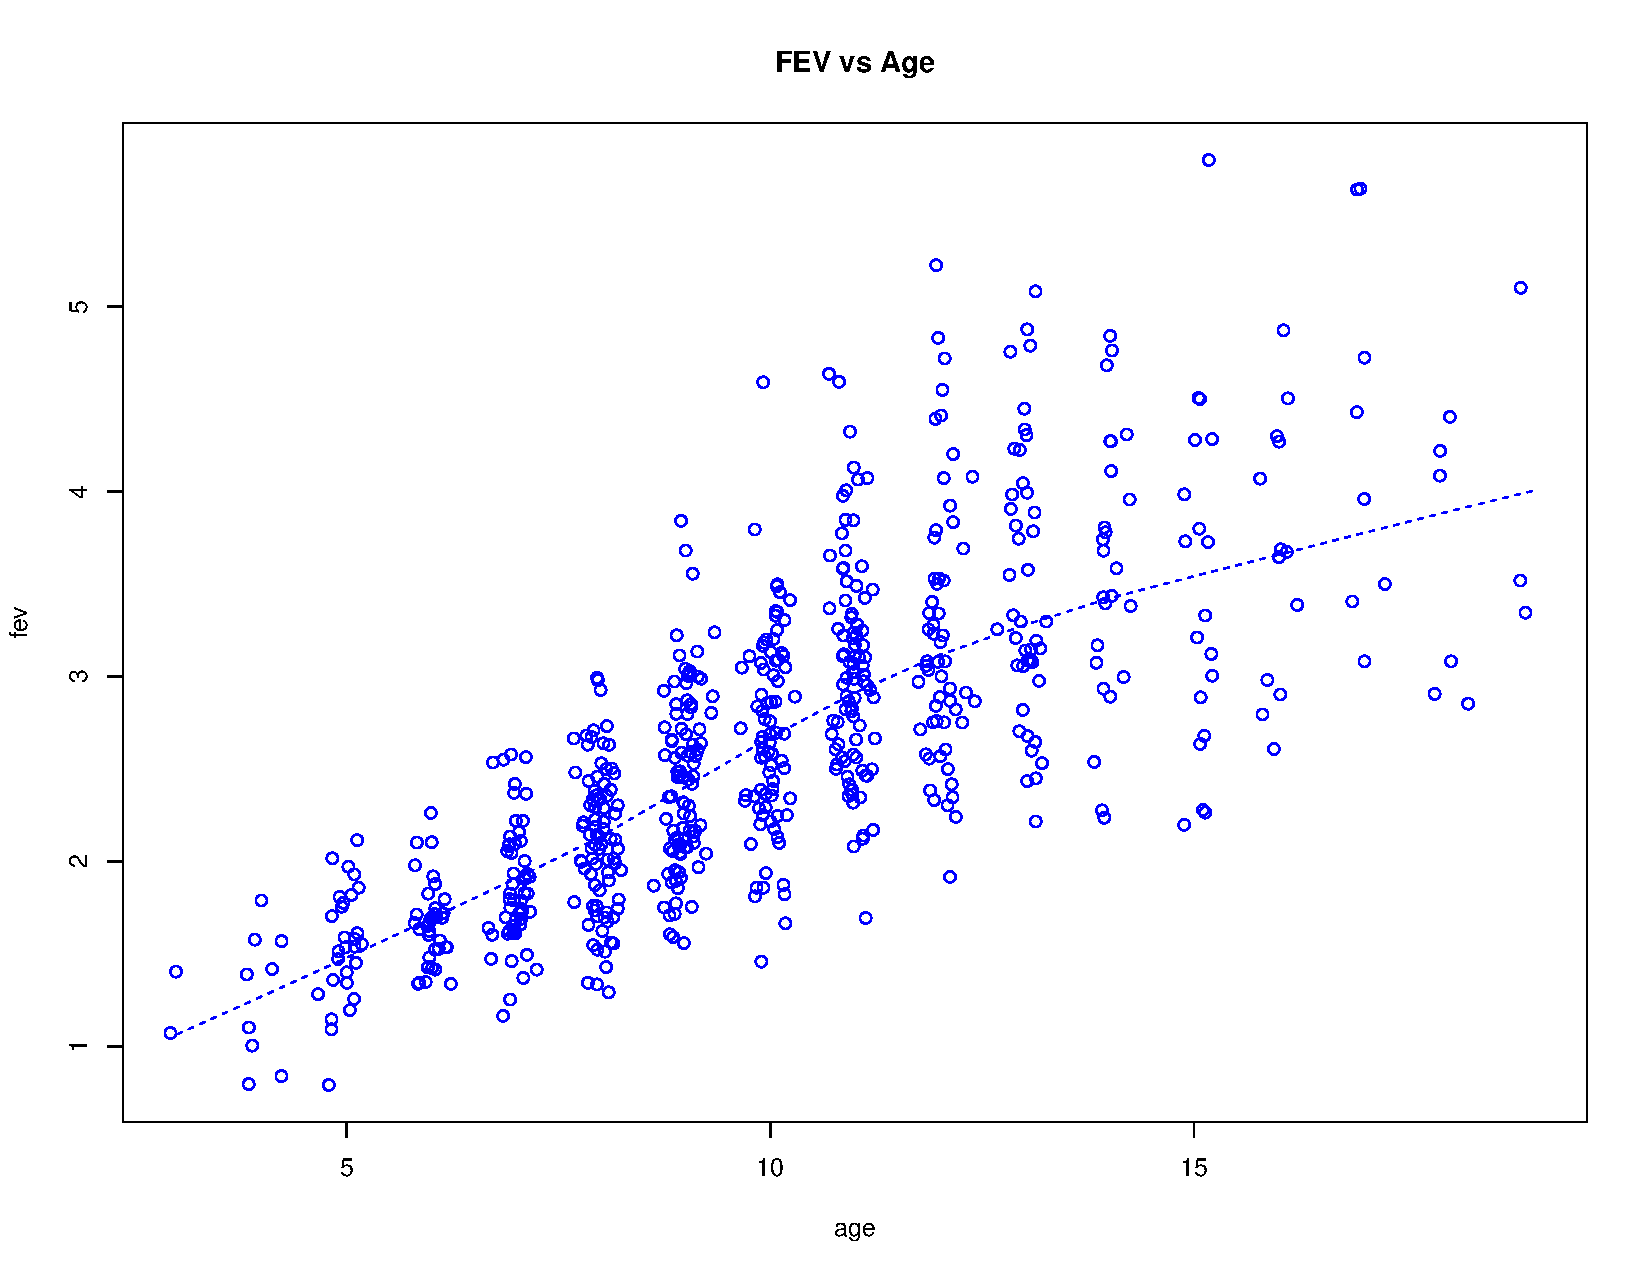
\includegraphics[scale=.005]{fevdoc-agefevscatter2}
\caption{Scatterplot of Age vs Height with lowess smooths}
\label{agefevscatter2}
\end{figure}
Now we can see a hint of an S-shaped trend in the data. We believe this, because if we believe that FEV is actually best predicted by height, then at young ages height is roughly linear with age but at older ages height is flat. In order to really understand what is going on, we must look at the relationship between FEV and height:\\
\begin{Schunk}
\begin{Sinput}
> scatter(fev, height, main="FEV vs Height")
\end{Sinput}
\end{Schunk}
\begin{figure}[h]
\centering
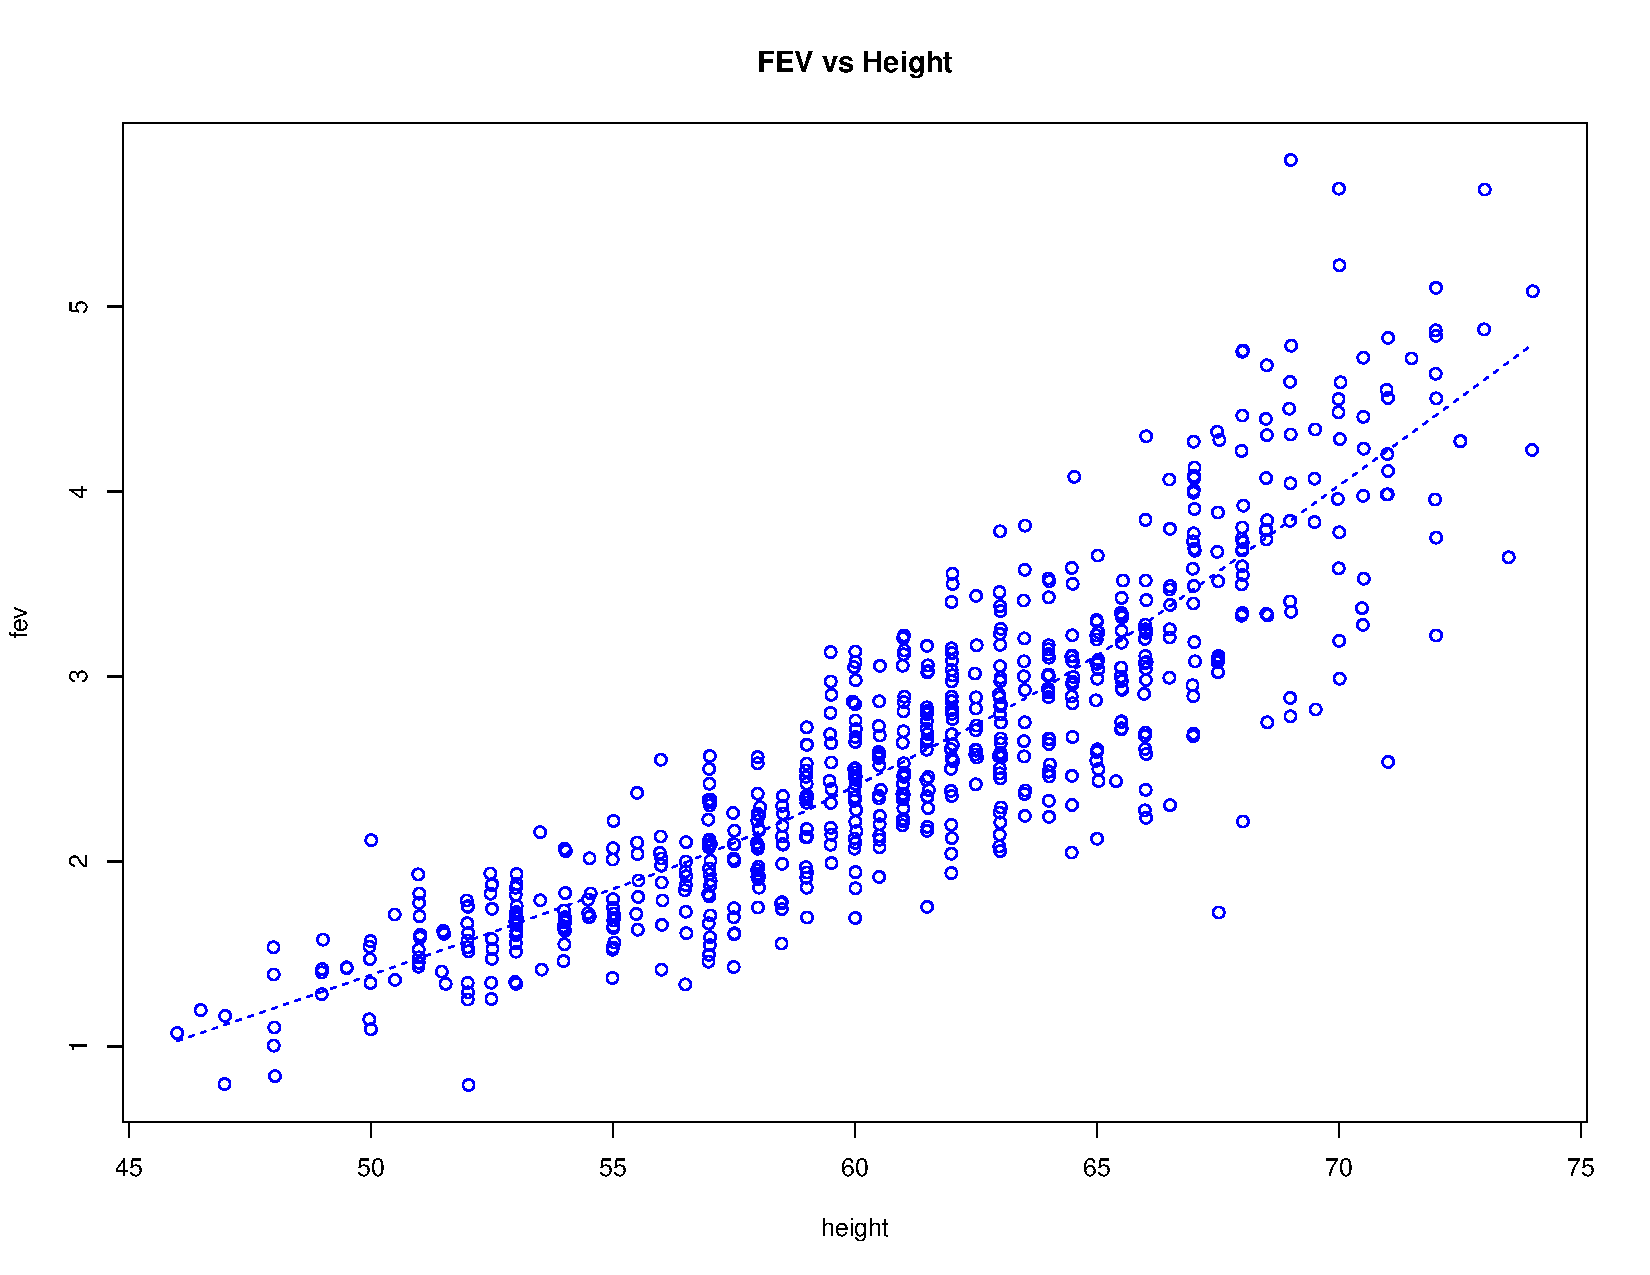
\includegraphics[scale=.005]{fevdoc-heightfevscatter1}
\caption{Scatterplot of FEV vs Height}
\label{heightfevscatter1}
\end{figure}
This is definitely not a linear relationship. In fact, it looks like a cubic relationship. Now if we look at the plot stratified by sex, we don't see too much of a sex effect:\\
\begin{Schunk}
\begin{Sinput}
> scatter(fev, height, strata=male, main="FEV vs Height by Sex")
\end{Sinput}
\end{Schunk}
\begin{figure}[h]
\centering
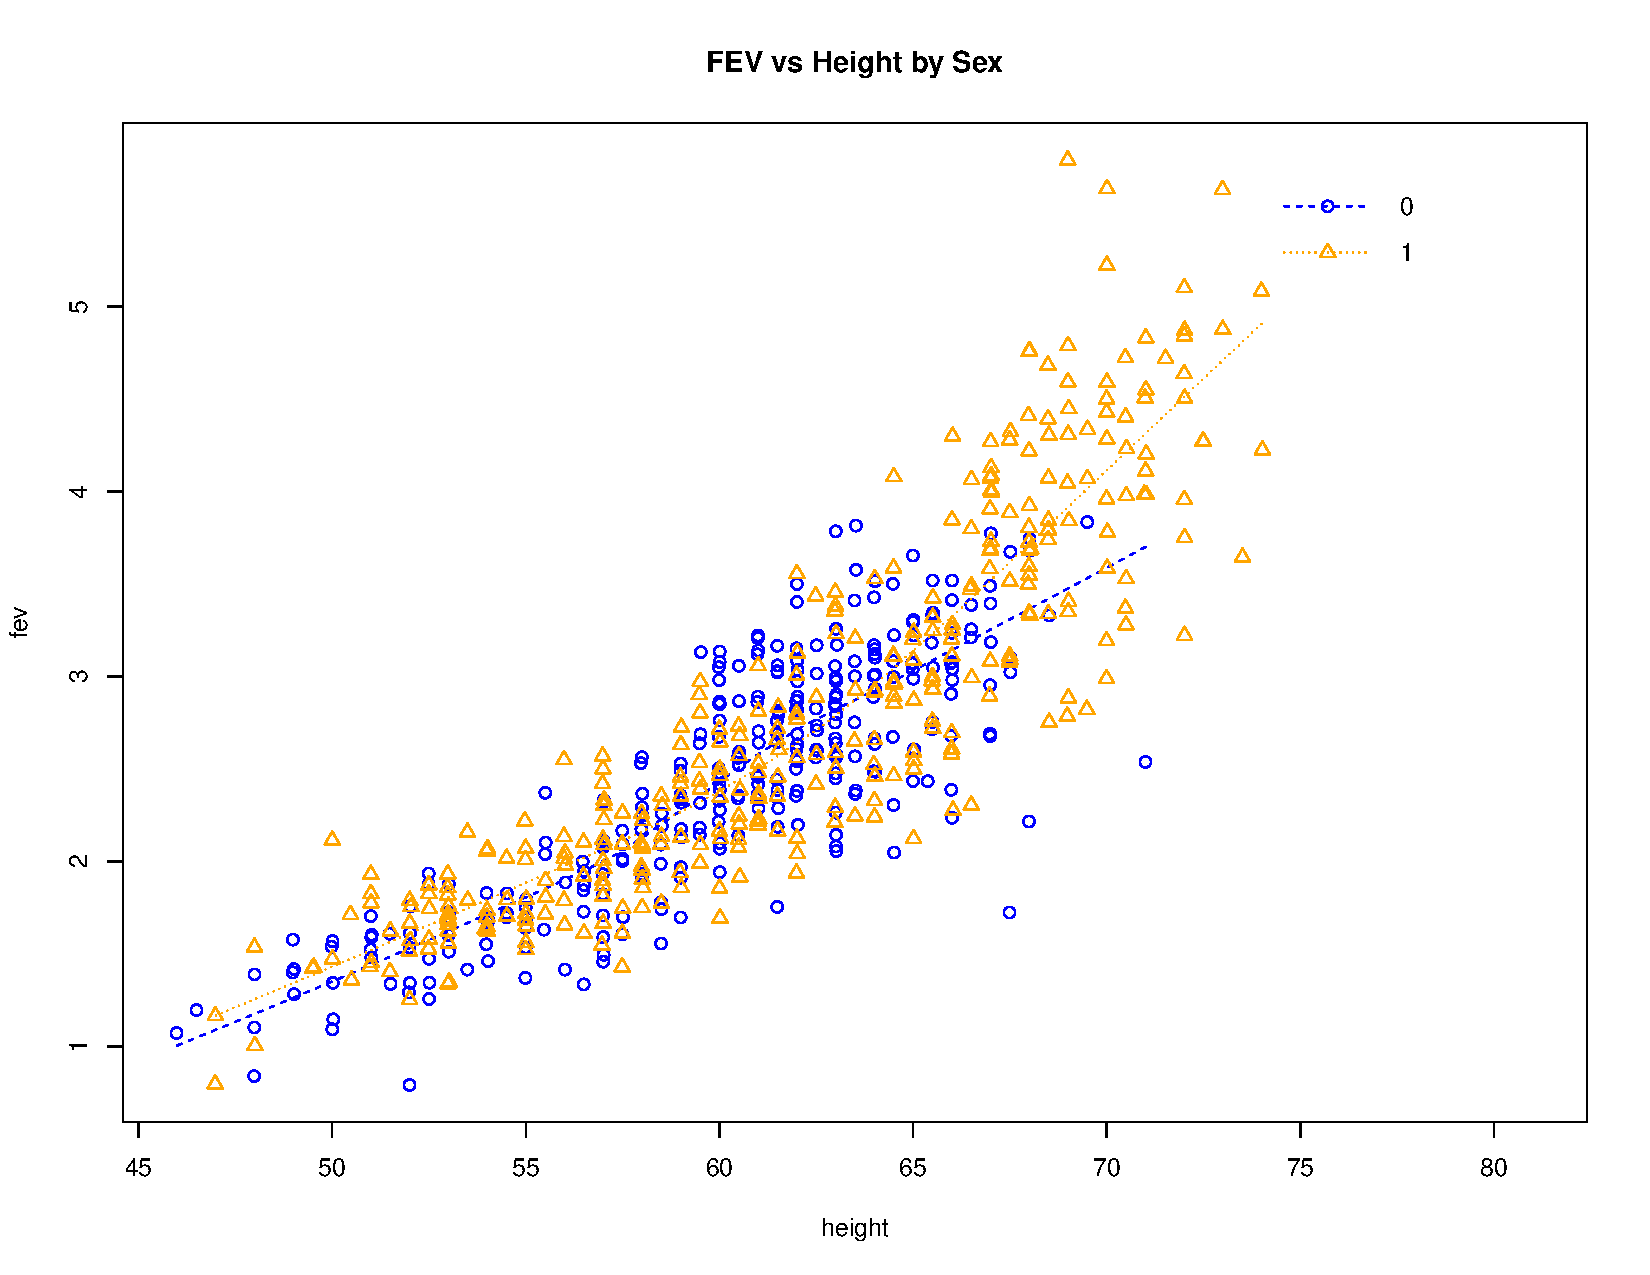
\includegraphics[scale=.005]{fevdoc-heightfevscatter2}
\caption{Scatterplot of FEV vs Height by Sex}
\label{heightfevscatter2}
\end{figure}
If we create a new variable called \texttt{htcub} (for height cubed) we can see that there is more of a straight line relationship with FEV:
\begin{Schunk}
\begin{Sinput}
> htcub <- height^3
> scatter(fev, htcub, main="FEV by Cubed Height")
\end{Sinput}
\end{Schunk}
\begin{figure}[h]
\centering
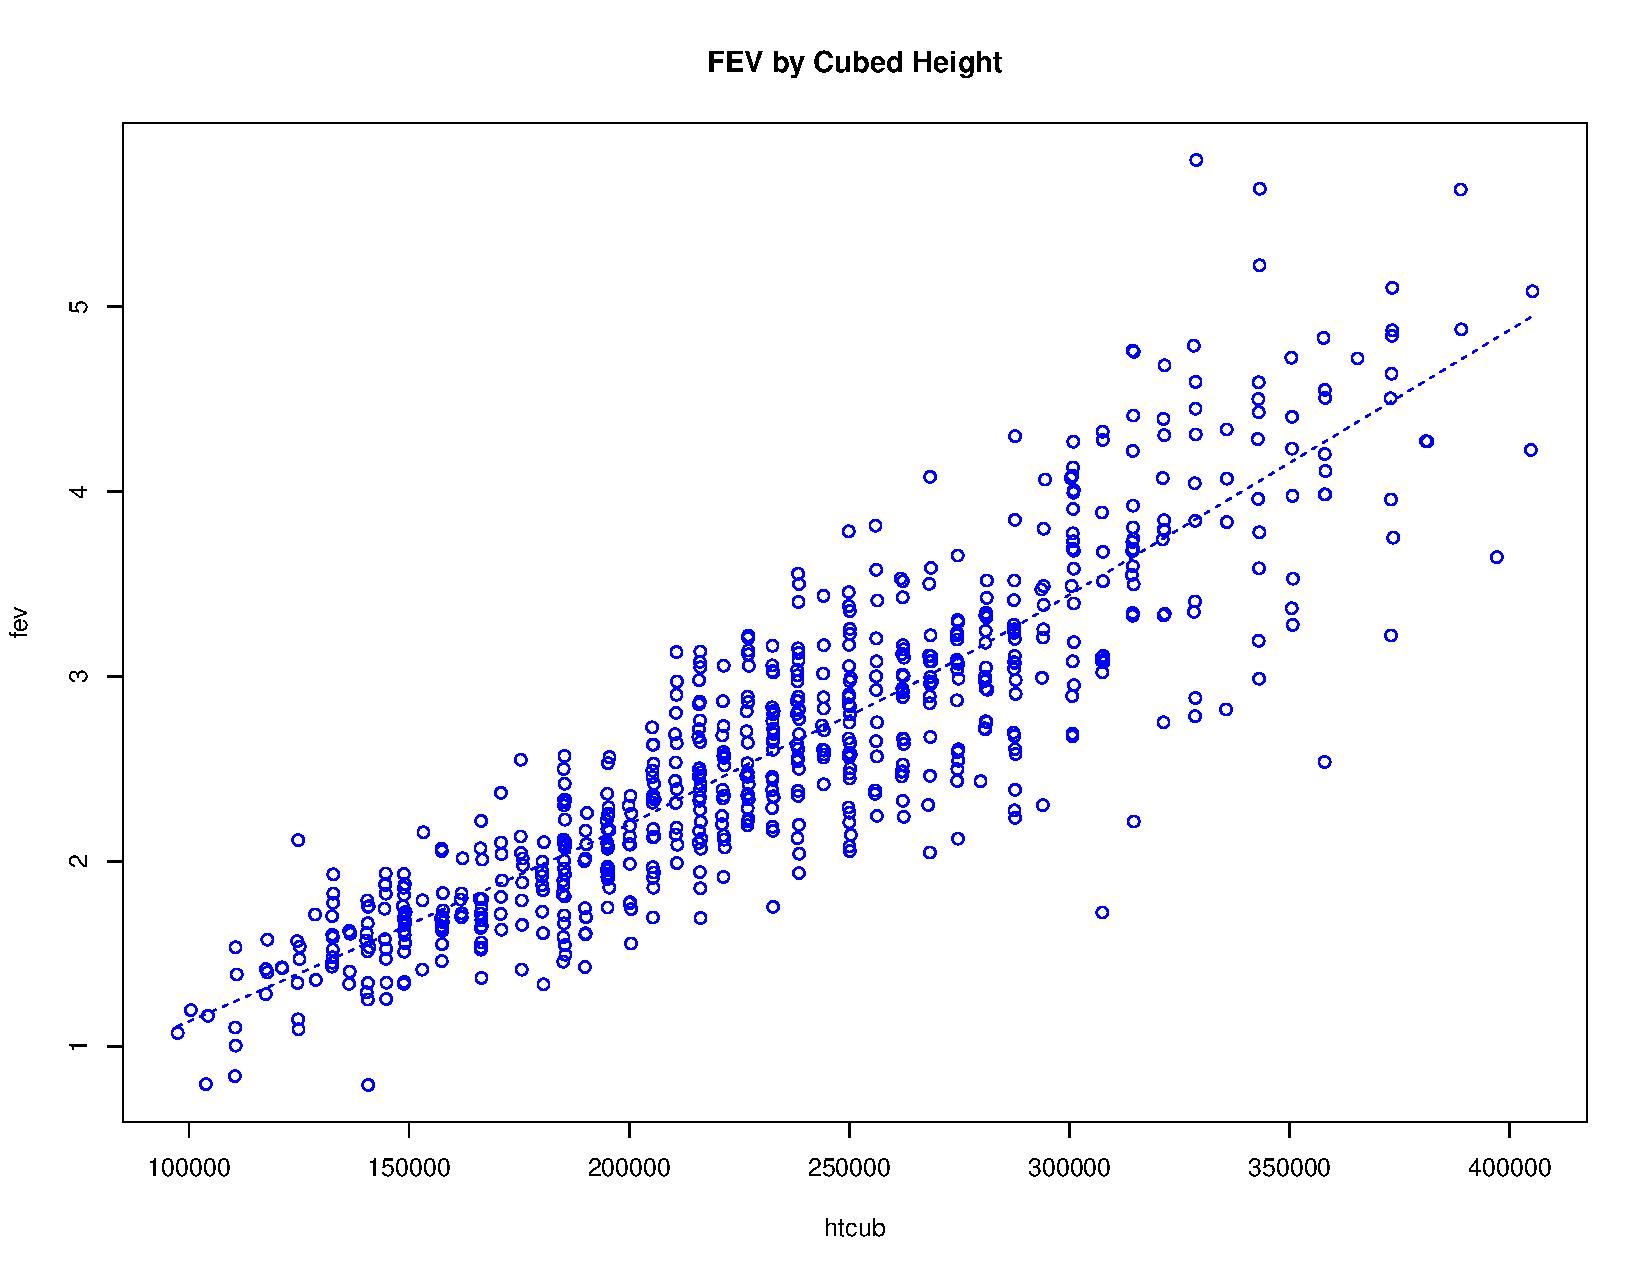
\includegraphics[scale=.005]{fevdoc-heightfevscatter3}
\caption{Scatterplot of Age vs Cubed Height}
\label{heightfevscatter3}
\end{figure}
There is still heteroscedasticity, however. To remedy this, we can try plotting the cube root of FEV vs Height:\\
\begin{Schunk}
\begin{Sinput}
> cubrtfev <- fev^(1/3)
> scatter(cubrtfev, height, main="Cube Root of FEV by Height")
\end{Sinput}
\end{Schunk}
\begin{Schunk}
\begin{Sinput}
> cubrtfev <- fev^(1/3)
> scatter(cubrtfev, height, main="Cube Root of FEV by Height")
\end{Sinput}
\end{Schunk}
\begin{figure}[h]
\centering
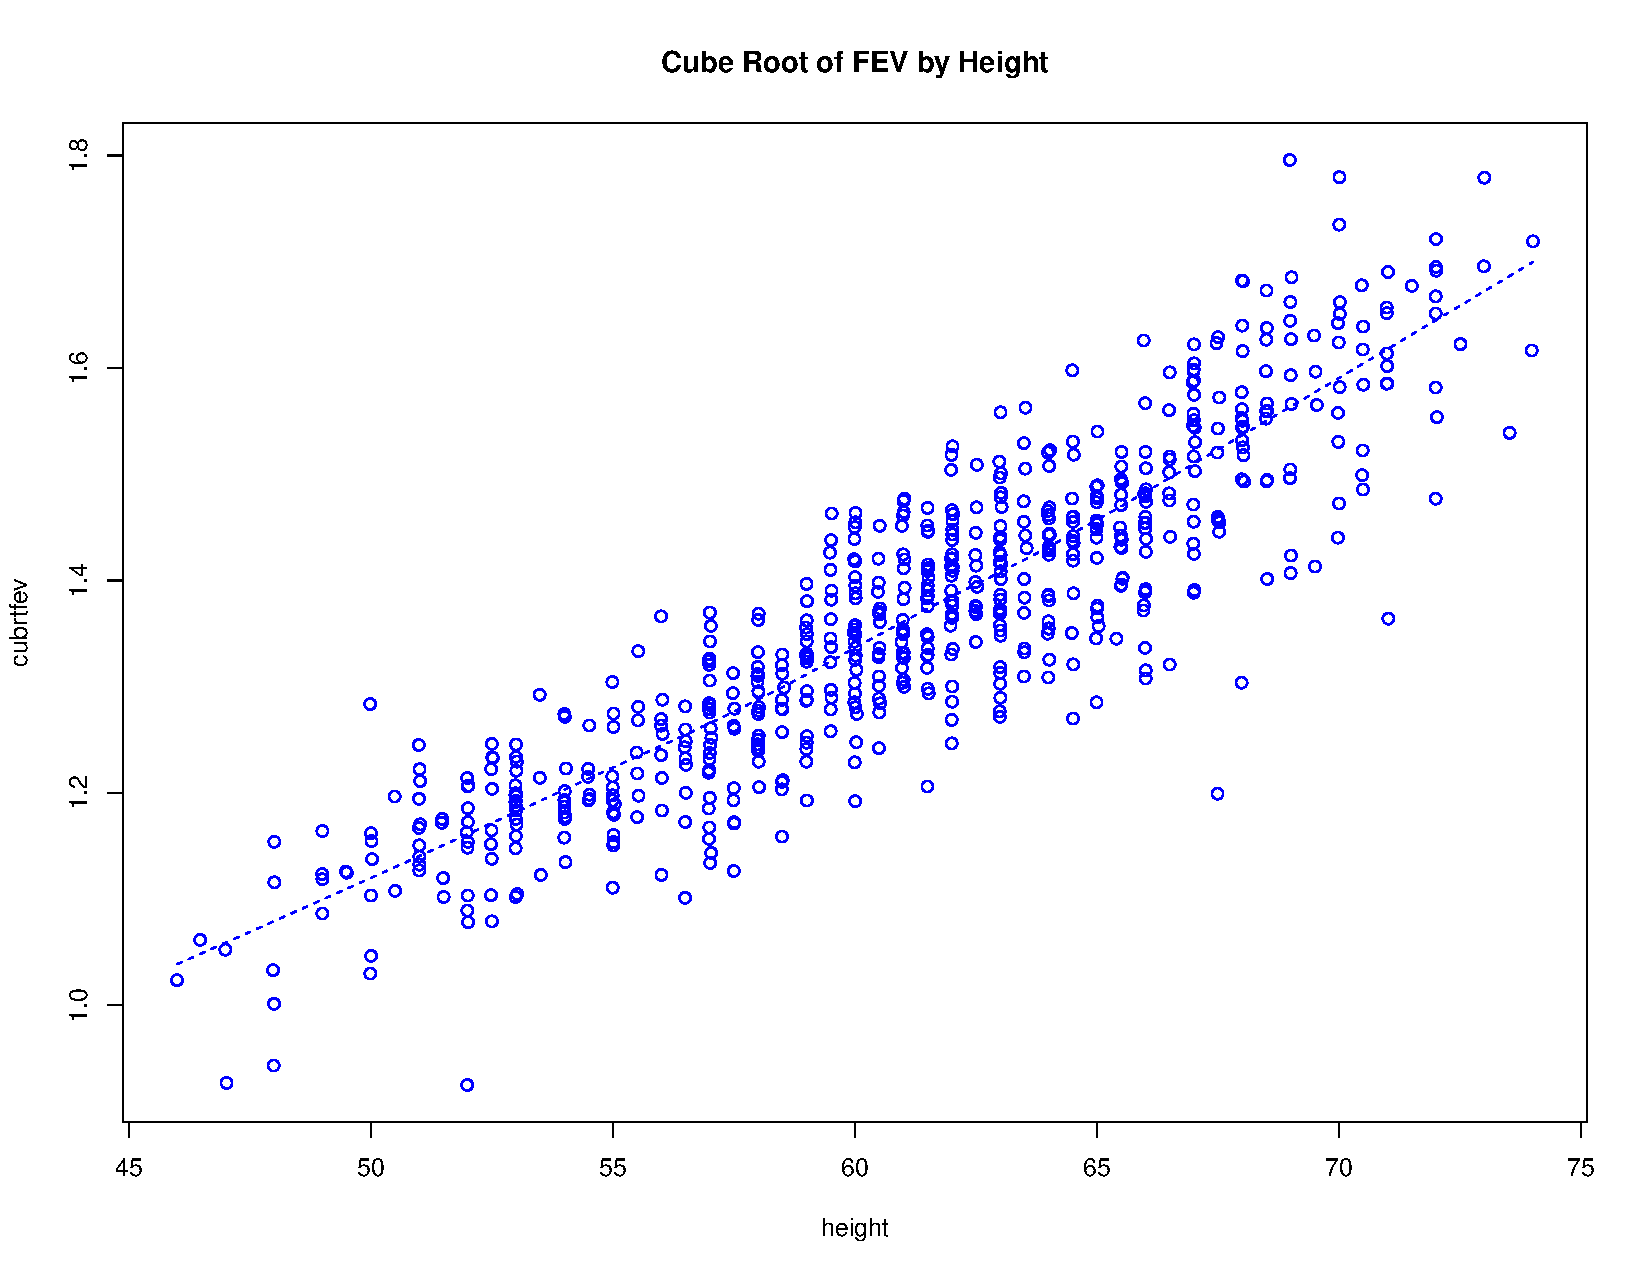
\includegraphics[scale=.005]{fevdoc-heightfevscatter4}
\caption{Scatterplot of Cube Root of FEV vs Height}
\label{heightfevscatter4}
\end{figure}
\clearpage
\section{The \texttt{fev} dataset revisited}
Now that we know all of these methods, what would we do if presented with the \texttt{fev} dataset? All of our data cleanup would happen immediately when we read in the data, based on the documentation and what we can see in R. 
\newline {\large \textbf{What do we want to do?}}
\newline \indent We want to read in the \texttt{fev} dataset and make it ready for use and analysis.
\newline {\large \textbf{How do we do that?}}
\newline \indent We first read in the dataset (renaming it as \texttt{fevDat} because we know that one of the variables in the data is named \texttt{fev} and we don't want confusion when we attach the data):
\begin{Schunk}
\begin{Sinput}
> fevDat <- read.table("http://www.emersonstatistics.com/Datasets/fev.txt", header=TRUE)
> attach(fevDat)
\end{Sinput}
\end{Schunk}
Now we view the data:
\begin{Schunk}
\begin{Sinput}
> View(fevDat)
\end{Sinput}
\end{Schunk}
After noticing that \texttt{sex} and \texttt{smoke} are not coded as indicator variables, we recode them (using the documentation online for reference):
\begin{Schunk}
\begin{Sinput}
> male <- ifelse(sex==1, 1, 0)
> smoker <- ifelse(smoke==2, 0, 1)
\end{Sinput}
\end{Schunk}
We also would know which variables are likely confounders or effect modifiers before starting the data analysis. Good practice in statistics dictates the choice of these variables before analysis, so that we are not using our data for exploratory purposes when we want to do inference. \newline
{\large \textbf{Interpretation}}
\newline \indent Now we have loaded the dataset, cleaned it up, and know what our confounding variables and effect modifiers are. Now we are ready to create plots and run our analysis.
\end{document}
